\documentclass[conference]{IEEEtran}

% ---------------------------------------------------------------------------
% Core Packages
% ---------------------------------------------------------------------------
\usepackage[utf8]{inputenc}
\usepackage[T1]{fontenc}
\usepackage{amsmath, amssymb, amsfonts}
\usepackage{graphicx}
\usepackage{booktabs}
\usepackage{multirow}
\usepackage{array}
\usepackage{url}
\usepackage{cite}
\usepackage{tikz}
\usepackage{algorithm}
\usepackage{algpseudocode}
\usepackage{caption}
\usepackage{subcaption}

% TikZ Libraries
\usetikzlibrary{positioning, shapes.geometric, arrows.meta, calc, fit}

% IEEE Citation and Reference Formatting
\def\BibTeX{{\rm B\kern-.05em{\sc i\kern-.025em b}\kern-.08em
    T\kern-.1667em\lower.7ex\hbox{E}\kern-.125emX}}

\begin{document}

% ---------------------------------------------------------------------------
% Title and Authors
% ---------------------------------------------------------------------------
\title{UrbanVending AI: A Geospatial Decision-Support and Micro-Allocation Framework for Municipal Street Vendor Zoning Using Multi-Criteria Evaluation, AHP Calibration, and Pre-emptive Goal Programming}

\author{
    \IEEEauthorblockN{Author Name 1\IEEEauthorrefmark{1}, Author Name 2\IEEEauthorrefmark{1}, Author Name 3\IEEEauthorrefmark{1}, and Author Name 4\IEEEauthorrefmark{1}}
    \IEEEauthorblockA{\IEEEauthorrefmark{1}Department of Information Technology\\
    [TODO: Insert College / Department Name], Nashik, Maharashtra, India\\
    Email: \{author1, author2, author3, author4\}@[TODO: institution domain]}
}

\maketitle

% ---------------------------------------------------------------------------
% Abstract and Index Terms
% ---------------------------------------------------------------------------
\begin{abstract}
Street vending sustains informal urban livelihoods across developing economies while supplying affordable goods to millions of city residents. However, uncoordinated street vending frequently conflicts with municipal infrastructure, causing pedestrian walkway encroachments, vehicular congestion, and public right-of-way disputes. Although statutory frameworks such as India's Street Vendors Act, 2014 mandate the demarcation of vending zones, municipal authorities lack operational geospatial tools to evaluate zone suitability, enforce carrying capacity, and engineer micro-scale physical vendor pitches. This paper presents UrbanVending AI, an end-to-end geospatial decision-support and micro-allocation framework for municipal street vendor zoning. Evaluated on official datasets from the Nashik Municipal Corporation (NMC) comprising 7,259 registered vendors and 308 municipal zones across six administrative divisions, the framework combines OpenStreetMap GIS feature engineering with unsupervised $K$-Means clustering ($ARI = 1.0$). A six-factor Multi-Criteria Decision Analysis (MCDA) engine incorporates non-linear saturation scaling, exponential proximity decay, and empirical Bayes category shrinkage with leave-location-group-out validation, calibrated via the Analytic Hierarchy Process (AHP) ($CR \le 0.10$). In a 224-scenario sensitivity audit, the MCDA model demonstrated 100\% Top-1 stability and a mean Spearman rank correlation of $\rho = 0.9977$. To resolve the spatial capacity paradox where greedy suitability selection causes massive over-allocation, the framework formulates two-stage pre-emptive Goal Programming (MILP) guaranteeing zero capacity violation. Physical feasibility is established through a metric micro-slot packing generator validated on the Lekha Nagar pilot (Zone NN\_F\_013), packing 10 standardized $2\,\text{m}\times 2\,\text{m}$ slots ($1.87 \times 10^{-9}\,\text{m}$ edge error) with $1.2\,\text{m}$ pedestrian clearance. Supervised benchmarking confirms that Random Forest regression ($R^2 = 0.7592$) achieves a 59.8\% error reduction over baselines, with TreeSHAP explainability attributing primary importance to commercial footfall. The operational system features an authenticated React/FastAPI architecture with HMAC-SHA256 identity hashing and direct Meta WhatsApp Cloud API integration, providing an auditable, privacy-preserving solution for equitable urban governance.
\end{abstract}

\begin{IEEEkeywords}
Geographic Information Systems (GIS), Multi-Criteria Decision Analysis (MCDA), Analytic Hierarchy Process (AHP), Pre-emptive Goal Programming, Mixed-Integer Linear Programming (MILP), Urban Street Vending, Micro-Slot Allocation, Explainable AI (XAI), TreeSHAP.
\end{IEEEkeywords}

% ---------------------------------------------------------------------------
% Main Content Sections
% ---------------------------------------------------------------------------
\section{Introduction}
\label{sec:introduction}

Street vending constitutes a vital socioeconomic pillar in developing and emerging urban economies. Across the Global South, millions of micro-entrepreneurs rely on informal retail to sustain household livelihoods, while urban residents depend on street vendors for affordable, proximate access to fresh produce, prepared food, and essential commodities~\cite{bhowmik2005street, bromley2000street}. However, the rapid expansion of informal vending often collides with formal municipal infrastructure, generating severe urban governance tensions. In dense commercial nodes, unregulated vending can lead to pedestrian walkway encroachments, vehicular gridlock, visual disorder, and acute sanitation deficiencies~\cite{bromley2000street}. Conversely, heavy-handed eviction policies and punitive clearances undermine the statutory protections granted to vulnerable vendors, precipitating immediate livelihood precarity.

To institutionalize a rights-based regulatory framework, statutory mandates such as the \textit{Street Vendors (Protection of Livelihood and Regulation of Street Vending) Act, 2014} in India established legal mechanisms to protect vendors from arbitrary displacement while mandating Urban Local Bodies (ULBs) to delineate designated vending, restricted vending, and non-vending zones~\cite{india2014street}. In practice, however, municipal authorities face formidable computational and operational hurdles when attempting to implement these legal mandates at scale.

\subsection{The Unverified Heuristic Allocation Challenge}
\label{sec:unverified_challenge}

In most municipal jurisdictions, including the Nashik Municipal Corporation (NMC) in Maharashtra, India, street vendor zoning and permit allocations have historically relied on static paper-based registries, coarse town-planning maps, or uncoordinated discretionary officer decisions. Such traditional approaches suffer from three systemic vulnerabilities:

\begin{enumerate}
    \item \textbf{Spatial and Environmental Blindness:} Conventional zone categorization assigns arbitrary capacity ceilings without quantitative spatial analysis of local pedestrian accessibility, transit connectivity, or proximity to critical amenities such as public sanitary conveniences and water infrastructure.
    \item \textbf{Category-Zone Incompatibility and Disagreement:} Retail requirements vary drastically across business typologies. A perishable produce vendor requires different proximity characteristics and waste facilities than an apparel or dry-goods cart. Heuristic assignments routinely locate vendors in commercial deserts or in over-saturated clusters where excessive competition induces financial insolvency.
    \item \textbf{The Aggregate Capacity Paradox:} Even when a high-level zoning plan specifies aggregate zone capacities, municipal systems lack physical micro-allocation mechanisms. In practice, vendors assigned to a designated zone compete chaotically for curb space, frequently encroaching on mandatory pedestrian corridors and roadway clear zones. Furthermore, predictive machine learning models, if deployed naively, risk assigning vendors to high-suitability locations that are already over-saturated, thereby violating statutory physical space constraints.
\end{enumerate}

\subsection{Project Objectives and Research Contributions}
\label{sec:objectives}

To bridge the gap between statutory zoning mandates and operational urban execution, this paper presents \textbf{UrbanVending AI}, an end-to-end geospatial decision-support and micro-allocation framework engineered for municipal street vendor governance. The framework integrates multi-source geographic information systems (GIS), unsupervised spatial clustering, missing-data-aware Multi-Criteria Decision Analysis (MCDA), Analytic Hierarchy Process (AHP) calibration, pre-emptive Goal Programming, and metric micro-slot packing.

The principal technical contributions of this work are as follows:

\begin{itemize}
    \item \textbf{Comprehensive Municipal GIS Ingestion Pipeline:} Ingestion, normalization, and geographic reconciliation of 7,259 official vendor records and 308 municipal zones across six administrative divisions of Nashik, cross-referenced with 13,988 road geometries and 353 commercial point-of-interest (POI) clusters from OpenStreetMap (OSM).
    \item \textbf{Environmental Typology via Spatial Clustering:} Unsupervised $K$-Means modeling on 12 scale-transformed environmental features across 258 usable zone geometries, establishing a reproducible environmental baseline ($ARI = 1.0$ across random initialization seeds).
    \item \textbf{Missing-Data-Aware MCDA with AHP Calibration:} A six-factor decision-support engine incorporating non-linear log-saturation, exponential proximity decay, and empirical Bayes category shrinkage with leave-location-group-out cross-validation to prevent self-reinforcing historical bias, calibrated via AHP with formal consistency ratio verification ($CR \le 0.10$).
    \item \textbf{Robustness via Large-Scale Sensitivity Analysis:} Comprehensive evaluation across 224 weight-perturbation scenarios, proving 100\% Top-1 ranking stability and a mean Spearman rank correlation of $\rho = 0.9977$.
    \item \textbf{Two-Stage Pre-emptive Goal Programming (MILP):} A mathematical optimization formulation solved via the HiGHS dual revised simplex engine that guarantees zero capacity over-allocation while minimizing vendor suitability loss and preference fallback.
    \item \textbf{Metric Micro-Slot Packing Generator:} Geographic micro-allocation in projected metric coordinates (EPSG:32643 / UTM Zone 43N), validated on the Lekha Nagar (NN\_F\_013) pilot to pack 10 standardized $2\,\text{m} \times 2\,\text{m}$ slots with sub-millimeter edge tolerances, $\ge 0.5\,\text{m}$ spacing, and a $1.2\,\text{m}$ continuous pedestrian corridor.
    \item \textbf{Explainable ML Suitability Benchmarking:} Supervised benchmarking across 5-fold grouped cross-validation, demonstrating that ensemble regression ($R^2 = 0.7592$, $\text{MAE} = 0.2469$) outperforms mean baselines by 59.8\%, accompanied by TreeSHAP feature attributions.
    \item \textbf{Production Full-Stack Architecture with Privacy Guardrails:} An authenticated, role-based platform pairing a React/Leaflet dashboard with a FastAPI/SQLite backend, featuring HMAC-SHA256 identity hashing for vendor privacy and direct Meta WhatsApp Cloud API integration.
\end{itemize}

\subsection{Paper Organization}
\label{sec:org}

The remainder of this paper is structured as follows. Section~\ref{sec:literature_review} surveys related literature in urban informal economics, spatial MCDA, mathematical programming, and explainable AI. Section~\ref{sec:methodology} formalizes the seven-stage UrbanVending AI methodology and mathematical formulations. Section~\ref{sec:experimental_setup} outlines the empirical datasets and evaluation metrics. Section~\ref{sec:results} presents experimental findings, sensitivity analyses, pilot micro-slot validation, and ablation studies. Section~\ref{sec:implementation} details the operational software architecture and conversational integration. Section~\ref{sec:discussion} discusses policy implications, threats to validity, and limitations. Finally, Section~\ref{sec:conclusion} concludes the paper and delineates future research directions.

\section{Literature Review}
\label{sec:literature_review}

Urban street vending management lies at the confluence of urban geography, informal economics, multi-criteria spatial modeling, operations research, and interpretable machine learning. This section reviews relevant theoretical and empirical foundations, highlighting key limitations in prior approaches that motivate the proposed framework.

\subsection{Street Vending Governance and Informal Urban Economics}
\label{sec:lit_vending}

In their seminal reviews of street vending across Asia and Latin America, Bhowmik~\cite{bhowmik2005street} and Bromley~\cite{bromley2000street} established that the informal retail sector is neither a transient friction nor an inherently parasitic phenomenon. Instead, it constitutes an indispensable structural element of urban consumer distribution, absorbing significant labor surpluses and supplying low-income urban strata with essential food and household commodities. However, uncoordinated vending generates spatial externalities, including footway impedance, public right-of-way contestation, and vehicular congestion. 

In India, recognition of these dynamics culminated in the \textit{Street Vendors (Protection of Livelihood and Regulation of Street Vending) Act, 2014}, which legally established Town Vending Committees (TVCs) and mandated spatial surveys, natural market demarcation, and periodic socio-economic census enumeration~\cite{india2014street}. Despite this progressive legislative mandate, municipal authorities frequently encounter operational deficits: zoning decisions are often negotiated through blunt administrative decrees or static tabular records lacking fine-grained spatial evidence.

\subsection{Spatial Multi-Criteria Decision Analysis and AHP in Urban Planning}
\label{sec:lit_mcda}

Multi-Criteria Decision Analysis (MCDA) integrated with Geographic Information Systems (GIS) provides a rigorous mathematical apparatus for evaluating competing spatial alternatives~\cite{malczewski1999gis}. Malczewski~\cite{malczewski2006ordered} demonstrated that spatial decision-making fundamentally requires balancing heterogeneous environmental attributes—such as proximity to transport nodes, pedestrian density, and public infrastructure—where no single alternative simultaneously dominates all criteria.

To assign objective weights across criteria, the Analytic Hierarchy Process (AHP), formulated by Saaty~\cite{saaty1980analytic, saaty1990how}, has been widely adopted in municipal site-suitability studies. AHP decomposes complex multi-attribute decision problems into a reciprocal pairwise comparison matrix, calculating criterion weights via the principal eigenvector and bounding subjective inconsistencies through the Consistency Ratio ($CR$). 

However, conventional spatial MCDA pipelines assume complete spatial datasets and static uniform weights across all decision agents. In municipal street vendor allocation, criteria data are frequently incomplete or subject to varying spatial survey coverage. Moreover, existing systems rarely implement non-linear diminishing-returns transforms or shrinkage mechanisms to prevent historical self-reinforcement when measuring location-category compatibility.

\subsection{Mathematical Optimization and Goal Programming}
\label{sec:lit_optimization}

While spatial MCDA computes a suitability score for individual vendor-zone pairings, it does not solve the collective resource-allocation problem under strict municipal capacity constraints. When multiple vendors compete for limited authorized slots in prime commercial zones, independent greedy allocation based on MCDA scores inevitably causes catastrophic capacity over-allocation.

To resolve competing institutional objectives under finite resource constraints, Charnes and Cooper~\cite{charnes1977goal} introduced Goal Programming as an extension of linear programming. Romero~\cite{romero1991handbook} further developed pre-emptive (lexicographic) Goal Programming, wherein higher-priority organizational goals (e.g., maximizing the absolute number of legally accommodated vendors) are satisfied before subordinate optimization goals (e.g., minimizing suitability loss or preference fallback) are considered. 

Recent advancements in mathematical programming solvers, such as the open-source HiGHS solver~\cite{huang2023highs} integrated into SciPy~\cite{virtanen2020scipy}, enable efficient exact solutions to large-scale mixed-integer linear programming (MILP) allocation problems. However, the application of two-stage pre-emptive Goal Programming directly coupled with spatial MCDA suitability scores and physical geometric micro-slot packing remains largely unexplored in municipal street vending literature.

\subsection{Spatial Clustering and Open GIS Infrastructure}
\label{sec:lit_clustering}

The extraction of environmental typologies from urban spatial data relies on unsupervised clustering algorithms, with $K$-Means clustering~\cite{macqueen1967some, lloyd1982least} remaining the foundational benchmark for continuous multi-dimensional feature partitioning. 

With the maturation of collaborative geographic data platforms like OpenStreetMap (OSM)~\cite{haklay2008openstreetmap}, urban researchers can extract comprehensive physical road networks and commercial point-of-interest (POI) layers without proprietary geographic database licensing. Nevertheless, volunteer geographic information exhibits spatial reporting variability and missingness. Unsupervised clustering models must therefore be rigorously evaluated against random-seed stability and decoupled from legal allocation constraints to avoid treating unverified spatial clusters as statutory vending zones.

\subsection{Supervised Machine Learning and Explainable AI (XAI)}
\label{sec:lit_ml_xai}

Ensemble machine learning algorithms, notably Random Forests~\cite{breiman2001random} and Extreme Gradient Boosting (XGBoost)~\cite{chen2016xgboost}, have demonstrated superior predictive capability on complex, non-linear tabular datasets~\cite{pedregosa2011scikit}. When applied to urban suitability estimation, however, black-box ensemble algorithms complicate institutional adoption because municipal officers and affected vendors cannot inspect the underlying decision logic.

To alleviate opacity, post-hoc Explainable AI (XAI) frameworks based on cooperative game theory, specifically SHapley Additive exPlanations (SHAP)~\cite{lundberg2017unified}, compute additive feature attributions satisfying local accuracy, missingness, and consistency. In urban governance applications, SHAP enables auditability by revealing which specific environmental factors (e.g., commercial density versus transit proximity) drove a given suitability judgment.

\subsection{Research Gap and Positioning of UrbanVending AI}
\label{sec:lit_gap}

A critical synthesis of prior literature reveals three overarching gaps:
\begin{enumerate}
    \item \textbf{Decoupling of Suitability and Capacity:} Existing spatial recommendation engines rank zones in isolation without constraining aggregate assignments against physical municipal carrying capacity.
    \item \textbf{Absence of Physical Micro-Slot Engineering:} Macro-level zoning allocations rarely bridge the gap to micro-scale geometric layout, leaving assigned vendors without demarcated $2\,\text{m}\times 2\,\text{m}$ footprints or mandatory pedestrian clearance corridors.
    \item \textbf{Heuristic Weighting without Rigorous Sensitivity Auditing:} Practical municipal systems often apply ad-hoc criteria weights without empirical sensitivity testing to verify ranking robustness under stakeholder weight perturbation.
\end{enumerate}

UrbanVending AI directly addresses these shortcomings through a unified, end-to-end framework integrating multi-criteria GIS modeling, AHP consistency calibration, 224-scenario sensitivity analysis, pre-emptive Goal Programming, and metric micro-slot packing.

\section{Proposed Methodology}
\label{sec:methodology}

The UrbanVending AI framework is structured into a seven-stage computational pipeline that seamlessly bridges high-level municipal policy, spatial GIS intelligence, mathematical optimization, and physical micro-slot engineering. Fig.~\ref{fig:architecture} depicts the multi-tier system architecture, and Fig.~\ref{fig:workflow} illustrates the end-to-end allocation workflow.

\begin{figure*}[t]
    \centering
    % System Architecture Diagram in TikZ
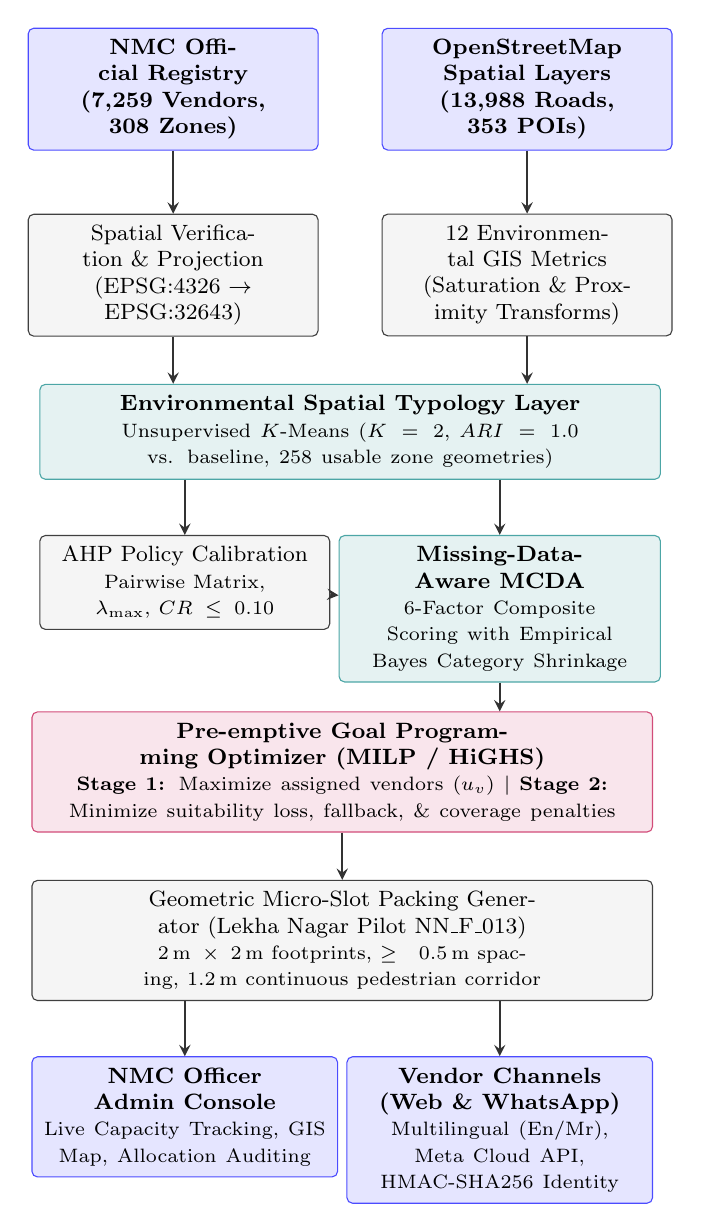
\begin{tikzpicture}[
    node distance=1.1cm and 1.2cm,
    box/.style={
        rectangle, draw=black!75, fill=gray!8, rounded corners=2pt,
        text centered, font=\footnotesize, minimum height=0.7cm, inner sep=4pt
    },
    primary/.style={
        box, fill=blue!10, draw=blue!70, font=\footnotesize\bfseries
    },
    accent/.style={
        box, fill=teal!10, draw=teal!70, font=\footnotesize\bfseries
    },
    opt/.style={
        box, fill=purple!10, draw=purple!70, font=\footnotesize\bfseries
    },
    layer/.style={
        rectangle, draw=black!40, dashed, rounded corners=4pt, inner sep=6pt, fill=black!2
    },
    arrow/.style={
        ->, >=stealth, thick, draw=black!80
    }
]

% Top Layer: Data Ingestion
\node[primary, text width=3.4cm] (nmc_data) {NMC Official Registry\\(7,259 Vendors, 308 Zones)};
\node[primary, text width=3.4cm, right=0.8cm of nmc_data] (osm_data) {OpenStreetMap Spatial Layers\\(13,988 Roads, 353 POIs)};

% Layer 2: Spatial Feature Engineering & Clustering
\node[box, text width=3.4cm, below=0.8cm of nmc_data] (geom_prep) {Spatial Verification \& Projection\\(EPSG:4326 $\to$ EPSG:32643)};
\node[box, text width=3.4cm, below=0.8cm of osm_data] (gis_feat) {12 Environmental GIS Metrics\\(Saturation \& Proximity Transforms)};

\node[accent, text width=7.6cm, below=0.6cm of $(geom_prep.south)!0.5!(gis_feat.south)$] (kmeans) {
    Environmental Spatial Typology Layer\\
    \normalfont{\scriptsize Unsupervised $K$-Means ($K=2$, $ARI=1.0$ vs. baseline, 258 usable zone geometries)}
};

% Layer 3: Decision Engine
\node[box, text width=3.4cm, below=0.7cm of kmeans.south west, anchor=north west] (ahp_engine) {
    AHP Policy Calibration\\
    \normalfont{\scriptsize Pairwise Matrix, $\lambda_{\max}$, $CR \le 0.10$}
};
\node[accent, text width=3.8cm, below=0.7cm of kmeans.south east, anchor=north east] (mcda_engine) {
    Missing-Data-Aware MCDA\\
    \normalfont{\scriptsize 6-Factor Composite Scoring with Empirical Bayes Category Shrinkage}
};

% Layer 4: Mathematical Optimization & Micro-Allocation
\node[opt, text width=7.6cm, below=0.7cm of $(ahp_engine.south)!0.5!(mcda_engine.south)$] (milp) {
    Pre-emptive Goal Programming Optimizer (MILP / HiGHS)\\
    \normalfont{\scriptsize \textbf{Stage 1:} Maximize assigned vendors ($u_v$) $\mid$ \textbf{Stage 2:} Minimize suitability loss, fallback, \& coverage penalties}
};

\node[box, text width=7.6cm, below=0.6cm of milp] (micro_alloc) {
    Geometric Micro-Slot Packing Generator (Lekha Nagar Pilot NN\_F\_013)\\
    \normalfont{\scriptsize $2\,\text{m}\times 2\,\text{m}$ footprints, $\ge 0.5\,\text{m}$ spacing, $1.2\,\text{m}$ continuous pedestrian corridor}
};

% Layer 5: Operational Delivery & Interfaces
\node[primary, text width=3.6cm, below=0.7cm of micro_alloc.south west, anchor=north west] (admin_ui) {
    NMC Officer Admin Console\\
    \normalfont{\scriptsize Live Capacity Tracking, GIS Map, Allocation Auditing}
};
\node[primary, text width=3.6cm, below=0.7cm of micro_alloc.south east, anchor=north east] (vendor_channel) {
    Vendor Channels (Web \& WhatsApp)\\
    \normalfont{\scriptsize Multilingual (En/Mr), Meta Cloud API, HMAC-SHA256 Identity}
};

% Arrows
\draw[arrow] (nmc_data) -- (geom_prep);
\draw[arrow] (osm_data) -- (gis_feat);
\draw[arrow] (geom_prep) -- (kmeans.north -| geom_prep);
\draw[arrow] (gis_feat) -- (kmeans.north -| gis_feat);

\draw[arrow] (kmeans.south -| ahp_engine) -- (ahp_engine);
\draw[arrow] (ahp_engine) -- (mcda_engine);
\draw[arrow] (kmeans.south -| mcda_engine) -- (mcda_engine);

\draw[arrow] (mcda_engine) -- (milp.north -| mcda_engine);
\draw[arrow] (milp) -- (micro_alloc);

\draw[arrow] (micro_alloc.south -| admin_ui) -- (admin_ui);
\draw[arrow] (micro_alloc.south -| vendor_channel) -- (vendor_channel);

\end{tikzpicture}

    \caption{Multi-tier system architecture of UrbanVending AI, spanning spatial data ingestion, environmental typology, AHP-calibrated MCDA, pre-emptive Goal Programming, and operational delivery.}
    \label{fig:architecture}
\end{figure*}

\begin{figure}[t]
    \centering
    % End-to-End Workflow Diagram in TikZ
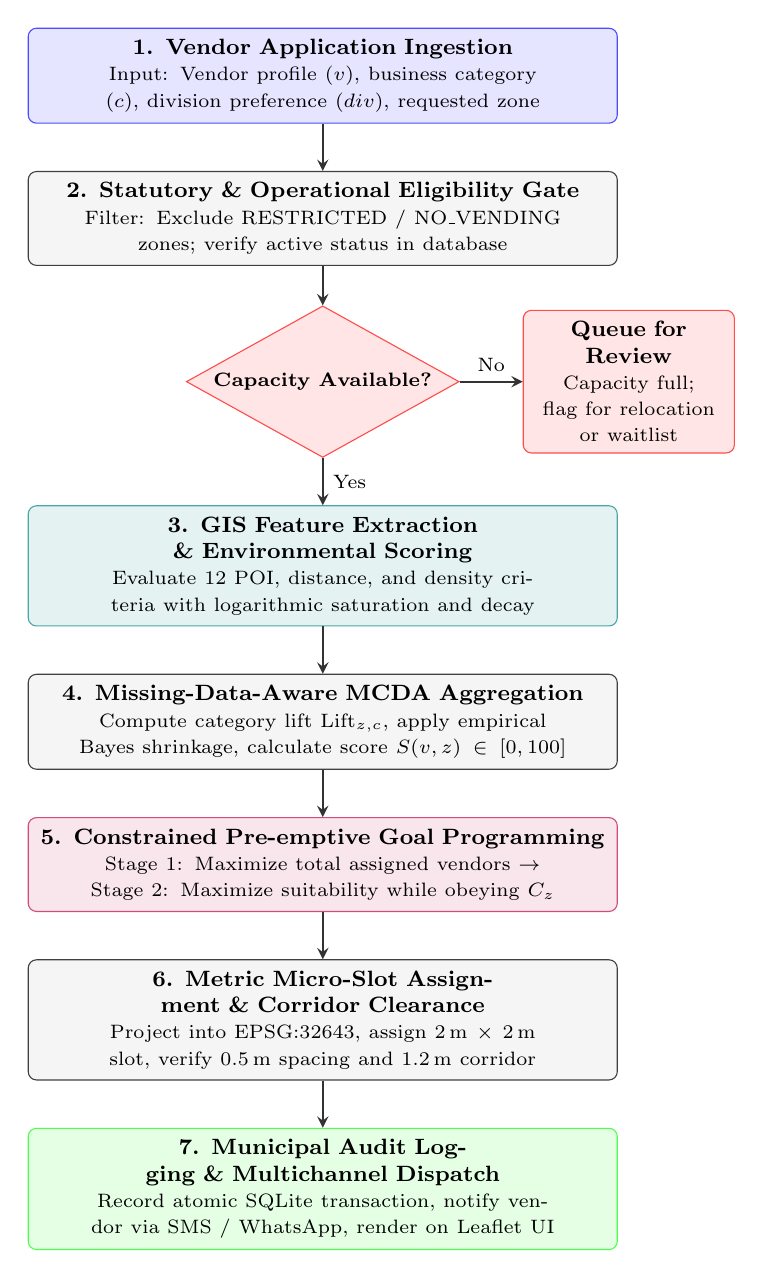
\begin{tikzpicture}[
    node distance=0.8cm,
    stepbox/.style={
        rectangle, draw=black!75, fill=gray!8, rounded corners=3pt,
        text centered, font=\footnotesize, minimum height=0.65cm, inner sep=4pt
    },
    decision/.style={
        diamond, draw=red!70, fill=red!10, text centered, font=\scriptsize\bfseries,
        inner sep=1.5pt, aspect=1.8
    },
    arrow/.style={
        ->, >=stealth, thick, draw=black!80
    }
]

% Steps
\node[stepbox, text width=7.2cm, fill=blue!10, draw=blue!70] (step1) {
    \textbf{1. Vendor Application Ingestion}\\
    \scriptsize Input: Vendor profile ($v$), business category ($c$), division preference ($div$), requested zone
};

\node[stepbox, text width=7.2cm, below=0.6cm of step1] (step2) {
    \textbf{2. Statutory \& Operational Eligibility Gate}\\
    \scriptsize Filter: Exclude RESTRICTED / NO\_VENDING zones; verify active status in database
};

\node[decision, below=0.5cm of step2] (dec1) {Capacity Available?};

\node[stepbox, text width=7.2cm, below=0.6cm of dec1, fill=teal!10, draw=teal!70] (step3) {
    \textbf{3. GIS Feature Extraction \& Environmental Scoring}\\
    \scriptsize Evaluate 12 POI, distance, and density criteria with logarithmic saturation and decay
};

\node[stepbox, text width=7.2cm, below=0.6cm of step3] (step4) {
    \textbf{4. Missing-Data-Aware MCDA Aggregation}\\
    \scriptsize Compute category lift $\text{Lift}_{z,c}$, apply empirical Bayes shrinkage, calculate score $S(v,z) \in [0, 100]$
};

\node[stepbox, text width=7.2cm, below=0.6cm of step4, fill=purple!10, draw=purple!70] (step5) {
    \textbf{5. Constrained Pre-emptive Goal Programming}\\
    \scriptsize Stage 1: Maximize total assigned vendors $\to$ Stage 2: Maximize suitability while obeying $C_z$
};

\node[stepbox, text width=7.2cm, below=0.6cm of step5] (step6) {
    \textbf{6. Metric Micro-Slot Assignment \& Corridor Clearance}\\
    \scriptsize Project into EPSG:32643, assign $2\,\text{m}\times 2\,\text{m}$ slot, verify $0.5\,\text{m}$ spacing and $1.2\,\text{m}$ corridor
};

\node[stepbox, text width=7.2cm, below=0.6cm of step6, fill=green!10, draw=green!70] (step7) {
    \textbf{7. Municipal Audit Logging \& Multichannel Dispatch}\\
    \scriptsize Record atomic SQLite transaction, notify vendor via SMS / WhatsApp, render on Leaflet UI
};

% Failure Node
\node[stepbox, text width=2.4cm, fill=red!10, draw=red!70, right=0.8cm of dec1] (reject) {
    \textbf{Queue for Review}\\
    \scriptsize Capacity full; flag for relocation or waitlist
};

% Connectors
\draw[arrow] (step1) -- (step2);
\draw[arrow] (step2) -- (dec1);
\draw[arrow] (dec1) -- node[right, font=\scriptsize] {Yes} (step3);
\draw[arrow] (dec1) -- node[above, font=\scriptsize] {No} (reject);
\draw[arrow] (step3) -- (step4);
\draw[arrow] (step4) -- (step5);
\draw[arrow] (step5) -- (step6);
\draw[arrow] (step6) -- (step7);

\end{tikzpicture}

    \caption{End-to-end allocation and micro-slot generation workflow, illustrating the operational gates and mathematical optimization stages.}
    \label{fig:workflow}
\end{figure}

\subsection{Stage 1: Multi-Source Municipal and Spatial Data Ingestion}
\label{sec:meth_stage1}

The pipeline ingests two primary data streams: (i) the official street vendor and zoning records from the Nashik Municipal Corporation (NMC), and (ii) urban road networks and point-of-interest (POI) spatial layers from OpenStreetMap (OSM).

Let $\mathcal{V} = \{v_1, v_2, \dots, v_N\}$ denote the set of $N = 7,259$ registered vendors, where each vendor $v$ is characterized by a tuple:
\begin{equation}
    v = \left( \text{ID}_v, c_v, d_v, \mathbf{x}_v, \text{Status}_v \right)
    \label{eq:vendor_tuple}
\end{equation}
where $c_v \in \mathcal{C}$ is the standardized business category, $d_v \in \mathcal{D}$ is the preferred administrative division, $\mathbf{x}_v$ represents historical location coordinates (if recorded), and $\text{Status}_v$ denotes registration status. The business category set $\mathcal{C}$ comprises:
\begin{equation}
    \mathcal{C} = \left\{ \text{vegetable\_fruit}, \text{food}, \text{clothing}, \text{flower}, \text{general\_goods}, \text{other} \right\}
    \label{eq:categories}
\end{equation}

Similarly, let $\mathcal{Z} = \{z_1, z_2, \dots, z_M\}$ denote the set of $M = 308$ official municipal vending zones across the six NMC administrative divisions $\mathcal{D} = \{\text{Nashik East}, \text{Nashik West}, \text{Nashik Road}, \text{Panchavati}, \text{CIDCO}, \text{Satpur}\}$. Each zone $z$ is characterized by:
\begin{equation}
    z = \left( \text{ID}_z, \text{Type}_z, C_z, \mathcal{P}_z \right)
    \label{eq:zone_tuple}
\end{equation}
where $\text{Type}_z \in \{\text{FREE}, \text{RESTRICTED}, \text{NO\_VENDING}\}$, $C_z \in \mathbb{N}_{\ge 0}$ is the authorized municipal capacity, and $\mathcal{P}_z$ represents the zone reference geometry. Among the 308 official zones, 258 possess verified usable reference geometries, while 50 lack usable geographic boundaries and are flagged for physical re-survey.

\subsection{Stage 2: Spatial Feature Engineering and Non-linear Transforms}
\label{sec:meth_stage2}

Raw spatial indicators, such as raw POI counts or distances in meters, exhibit heavy-tailed distributions and cannot be directly aggregated into linear multi-criteria models. UrbanVending AI applies two deterministic non-linear transformations:

\subsubsection{Logarithmic Saturation Transform}
For count and density metrics where additional units yield diminishing utility beyond an empirical saturation threshold $\beta > 0$, the feature value $x \in \mathbb{R}_{\ge 0}$ is transformed via:
\begin{equation}
    S(x, \beta) = \min\left(1.0, \frac{\ln(1 + \max(x, 0))}{\ln(1 + \beta)}\right)
    \label{eq:saturation}
\end{equation}
Table~\ref{tab:mcda_scales} lists the empirical saturation scaling parameters $\beta$ calibrated for commercial and public infrastructure criteria.

\subsubsection{Exponential Proximity Decay Transform}
For distance metrics where proximity represents positive utility and utility decays with physical displacement, the distance $d \ge 0$ (in meters) is transformed via:
\begin{equation}
    P(d, \lambda) = \exp\left( -\frac{\max(d, 0)}{\lambda} \right)
    \label{eq:proximity}
\end{equation}
where $\lambda > 0$ is the characteristic decay distance parameter.

\begin{table}[t]
    \caption{Scaling Parameters for Environmental Feature Transformations}
    \label{tab:mcda_scales}
    \centering
    \begin{tabular}{llr}
        \toprule
        \textbf{Criteria Factor} & \textbf{Feature Variable} & \textbf{Scale Parameter} \\
        \midrule
        \multirow{3}{*}{Commercial} & Commercial POI Count (250m) & $\beta = 12.0$ \\
                                   & Market POI Count (500m) & $\beta = 4.0$ \\
                                   & Food POI Count (250m) & $\beta = 8.0$ \\
        \midrule
        \multirow{3}{*}{Accessibility} & Distance to Major Road & $\lambda = 400.0\text{ m}$ \\
                                      & Distance to Bus Transit Access & $\lambda = 1000.0\text{ m}$ \\
                                      & Pedestrian Road Density (250m) & $\beta = 5000.0\text{ m/km}^2$ \\
        \midrule
        \multirow{4}{*}{Facilities}    & Healthcare Facility Count (500m) & $\beta = 15.0$ \\
                                      & Education Facility Count (500m) & $\beta = 6.0$ \\
                                      & Public Toilet Count (500m) & $\beta = 3.0$ \\
                                      & Public Parking Count (500m) & $\beta = 4.0$ \\
        \bottomrule
    \end{tabular}
\end{table}

\subsection{Stage 3: Unsupervised Environmental Typology (K-Means)}
\label{sec:meth_stage3}

To characterize the underlying spatial environment across the 258 usable zone geometries, the 12 normalized commercial, accessibility, and facility features are clustered using $K$-Means:
\begin{equation}
    \min_{\mathbf{\mu}} \sum_{k=1}^K \sum_{z \in \mathcal{C}_k} \|\mathbf{x}_z - \mathbf{\mu}_k\|_2^2
    \label{eq:kmeans}
\end{equation}
Cluster stability is benchmarked across five deterministic random seeds ($\{11, 23, 37, 53, 71\}$). Solutions for $K=2$ and $K=4$ are evaluated using the Adjusted Rand Index ($ARI$) and silhouette scores to partition zones into coherent environmental typologies without confusing unsupervised clusters with statutory zoning rules.

\subsection{Stage 4: Missing-Data-Aware Weighted MCDA}
\label{sec:meth_stage4}

The multi-criteria suitability engine evaluates six distinct criteria factors: Commercial Density ($f_{\text{com}}$), Accessibility ($f_{\text{acc}}$), Public Facilities ($f_{\text{fac}}$), Business Category Compatibility ($f_{\text{bus}}$), Preference Matching ($f_{\text{pref}}$), and Historical Association Density ($f_{\text{hist}}$).

\subsubsection{Empirical Bayes Category Compatibility with Leave-Group-Out Validation}
To determine how well zone $z$ accommodates business category $c$, the system avoids raw category proportions, which overfit small sample sizes. Let $n_z$ be the total historical vendors associated with zone $z$, $n_{z,c}$ be the count in category $c$, and $p_c = N_c / N_{\text{total}}$ be the citywide prior share. To eliminate self-reinforcing bias for an existing vendor $v$ possessing recorded location group $g_v$, the entire location group is removed from the estimation:
\begin{equation}
    n_{z}^{(-g_v)} = \sum_{v' \notin g_v, z(v') = z} 1, \quad n_{z,c}^{(-g_v)} = \sum_{v' \notin g_v, z(v') = z, c(v') = c} 1
    \label{eq:leave_group_out}
\end{equation}

The smoothed posterior category share $\hat{\theta}_{z,c}$ is computed via Laplace shrinkage with strength $M = 20.0$:
\begin{equation}
    \hat{\theta}_{z,c} = \frac{n_{z,c}^{(-g_v)} + M \cdot p_c}{n_z^{(-g_v)} + M}
    \label{eq:shrinkage}
\end{equation}
The historical category lift is defined as:
\begin{equation}
    \text{Lift}_{z,c} = \frac{\hat{\theta}_{z,c}}{p_c}
    \label{eq:lift}
\end{equation}
The business compatibility factor score $f_{\text{bus}}(z, c)$ scales the lift logarithmically while weighting by sample reliability:
\begin{equation}
    R(n_z) = \frac{n_z^{(-g_v)}}{n_z^{(-g_v)} + M}
    \label{eq:reliability}
\end{equation}
\begin{equation}
    f_{\text{bus}}(z, c) = 0.5 + \left( \min\left(1.0, \frac{\ln(1 + \max(\text{Lift}_{z,c}, 0))}{\ln(3)}\right) - 0.5 \right) \cdot R(n_z)
    \label{eq:f_bus}
\end{equation}
This formulation ensures that zones with negligible historical evidence revert to a neutral score of 0.5 rather than receiving an unmerited extreme penalty or bonus.

\subsubsection{Preference and Historical Density Scoring}
The preference factor $f_{\text{pref}}(v, z)$ scores 1.0 if zone $z$ belongs to vendor $v$'s preferred administrative division $d_v$, and 0.0 otherwise (or 0.5 if no preference is stated). Historical density is scored via saturation:
\begin{equation}
    f_{\text{hist}}(z) = S(n_z, 50.0)
    \label{eq:f_hist}
\end{equation}

\subsubsection{Missing-Data Renormalization}
Let $\mathcal{F} = \{\text{bus}, \text{com}, \text{acc}, \text{fac}, \text{pref}, \text{hist}\}$ index the six factors, and let $w_i > 0$ denote their calibrated weights with $\sum_{i \in \mathcal{F}} w_i = 1$. If a zone lacks data for factor $i$, the engine omits factor $i$ and renormalizes across available factors:
\begin{equation}
    \text{Score}(v, z) = 100 \times \frac{\sum_{i \in \mathcal{F}} w_i \cdot f_i(v, z) \cdot \mathbb{I}(f_i(v, z) \ne \text{NaN})}{\sum_{i \in \mathcal{F}} w_i \cdot \mathbb{I}(f_i(v, z) \ne \text{NaN})}
    \label{eq:mcda_aggregation}
\end{equation}
where $\mathbb{I}(\cdot)$ is the indicator function. The evidence coverage ratio is simultaneously tracked:
\begin{equation}
    \text{Coverage}(v, z) = \sum_{i \in \mathcal{F}} w_i \cdot \mathbb{I}(f_i(v, z) \ne \text{NaN}) \in [0, 1]
    \label{eq:coverage}
\end{equation}

\subsection{Stage 5: Analytic Hierarchy Process (AHP) Weight Calibration}
\label{sec:meth_stage5}

To establish credible baseline weights, an expert pairwise comparison matrix $\mathbf{A} \in \mathbb{R}^{6 \times 6}$ is constructed according to Saaty's 1–9 fundamental scale, where $a_{jk} = 1 / a_{kj}$ and $a_{jj} = 1$:
\begin{equation}
    \mathbf{A} \mathbf{w} = \lambda_{\max} \mathbf{w}
    \label{eq:ahp_eigen}
\end{equation}
The principal eigenvalue $\lambda_{\max}$ is calculated, and the Consistency Index ($CI$) and Consistency Ratio ($CR$) are computed via:
\begin{equation}
    CI = \frac{\lambda_{\max} - n}{n - 1}, \quad CR = \frac{CI}{RI(n)}
    \label{eq:cr}
\end{equation}
where $n = 6$ and $RI(6) = 1.24$. Pairwise comparison policies are accepted only if $CR \le 0.10$. The baseline policy establishes:
\begin{equation}
    \mathbf{w}_{\text{base}} = [w_{\text{bus}}=0.25, w_{\text{com}}=0.20, w_{\text{acc}}=0.20, w_{\text{fac}}=0.15, w_{\text{pref}}=0.10, w_{\text{hist}}=0.10]
    \label{eq:base_weights}
\end{equation}

\subsection{Stage 6: Two-Stage Pre-emptive Goal Programming Optimizer}
\label{sec:meth_stage6}

To allocate batches of vendors under strict municipal zone capacity limits without causing over-allocation, UrbanVending AI formulates a two-stage Mixed-Integer Linear Program (MILP) solved via the HiGHS dual simplex solver.

Let $x_{v,z} \in \{0, 1\}$ be the binary decision variable indicating whether vendor $v$ is assigned to zone $z$, and let $u_v \in \{0, 1\}$ indicate whether vendor $v$ remains unassigned.

\subsubsection{Stage 1: Cardinality Maximization}
The primary institutional goal of the municipality is to legally accommodate the maximum possible number of vendors (or equivalently, minimize unassigned vendors):
\begin{equation}
    \min_{\mathbf{x}, \mathbf{u}} \sum_{v \in \mathcal{V}} u_v
    \label{eq:milp_stage1}
\end{equation}
subject to:
\begin{align}
    \sum_{z \in \mathcal{Z}_{\text{elig}}} x_{v,z} + u_v &= 1, \quad \forall v \in \mathcal{V} \label{eq:con_vendor} \\
    \sum_{v \in \mathcal{V}} x_{v,z} &\le C_z, \quad \forall z \in \mathcal{Z} \label{eq:con_capacity} \\
    x_{v,z}, u_v &\in \{0, 1\}, \quad \forall v \in \mathcal{V}, z \in \mathcal{Z} \label{eq:con_binary}
\end{align}
where $\mathcal{Z}_{\text{elig}}$ denotes the set of legally OPEN zones possessing verified available capacity $C_z > 0$. Let $U^*$ denote the optimal objective value of Stage 1 (minimum unassigned vendors).

\subsubsection{Stage 2: Lexicographic Quality Optimization}
Holding the minimum unassigned count fixed at $U^*$, Stage 2 minimizes the composite penalty comprising suitability loss, preferred-division fallback, and low evidence coverage:
\begin{equation}
    \min_{\mathbf{x}, \mathbf{u}} \sum_{v \in \mathcal{V}} \sum_{z \in \mathcal{Z}_{\text{elig}}} x_{v,z} \cdot \Psi(v, z)
    \label{eq:milp_stage2}
\end{equation}
subject to (\ref{eq:con_vendor})--(\ref{eq:con_binary}) and the lexicographic constraint:
\begin{equation}
    \sum_{v \in \mathcal{V}} u_v = U^*
    \label{eq:con_lexicographic}
\end{equation}
where the edge penalty $\Psi(v, z)$ is defined as:
\begin{equation}
    \Psi(v, z) = (100 - \text{Score}(v, z)) + \alpha_{\text{fb}} \cdot \mathbb{I}(\text{Fallback}_{v,z}) + \alpha_{\text{cov}} \cdot (1 - \text{Coverage}(v, z))
    \label{eq:penalty}
\end{equation}
with default penalty coefficients $\alpha_{\text{fb}} = 0.10$ and $\alpha_{\text{cov}} = 0.05$.

\subsection{Stage 7: Metric Micro-Slot Packing Generator}
\label{sec:meth_stage7}

Once a zone is allocated, vendors require physically marked slots. Standard geographic representations in geographic coordinates (EPSG:4326) introduce severe latitude-dependent metric distortion. UrbanVending AI projects boundary polygons into metric projected coordinates (EPSG:32643 / UTM Zone 43N).

For each boundary polygon $\Omega \subset \mathbb{R}^2$, the generator determines the dominant orientation $\theta^*$ from the minimum rotated bounding rectangle:
\begin{equation}
    \theta^* = \arg\max_{\theta} \text{Length}(\text{Edge}(\text{MinRotatedRect}(\Omega)))
    \label{eq:orientation}
\end{equation}
Along this primary axis, the algorithm packs candidate square footprints of fixed dimension $w_{\text{slot}} \times h_{\text{slot}} = 2.0\,\text{m} \times 2.0\,\text{m}$. For each slot $k$, the generator enforces three geometric invariants:
\begin{align}
    \text{Footprint}_k &\subset \Omega \label{eq:geom_contain} \\
    \text{dist}(\text{Footprint}_k, \text{Footprint}_j) &\ge 0.50\text{ m}, \quad \forall j \ne k \label{eq:geom_spacing} \\
    \text{Corridor}(\Omega, w_{\text{corr}} = 1.2\text{ m}) &\cap \text{Footprint}_k = \emptyset, \quad \forall k \label{eq:geom_corridor}
\end{align}
Sub-millimeter numeric tolerances ($\le 0.002\,\text{m}$) are verified to guarantee that no physical obstruction or pedestrian right-of-way is violated.

\begin{algorithm}[t]
\caption{End-to-End UrbanVending AI Allocation Pipeline}
\label{alg:pipeline}
\begin{algorithmic}[1]
\Require Vendor demands $\mathcal{V}$, Zone registry $\mathcal{Z}$, Spatial features $\mathbf{X}_{\text{GIS}}$
\Ensure Optimal allocation plan $\mathbf{X}^*$ and physical slot coordinates $\mathcal{S}$
\State Filter candidate zones: $\mathcal{Z}_{\text{elig}} \gets \{z \in \mathcal{Z} \mid \text{Type}_z = \text{FREE} \land C_z > 0\}$
\For{each vendor $v \in \mathcal{V}$}
    \State Extract category $c_v$ and preferred division $d_v$
    \For{each zone $z \in \mathcal{Z}_{\text{elig}}$}
        \State Compute $\text{Lift}_{z,c_v}$ via leave-group-out shrinkage (Eq.~\ref{eq:leave_group_out}--\ref{eq:shrinkage})
        \State Compute non-linear feature scores $f_{\text{com}}, f_{\text{acc}}, f_{\text{fac}}$ (Eq.~\ref{eq:saturation}--\ref{eq:proximity})
        \State Calculate $\text{Score}(v,z)$ and $\text{Coverage}(v,z)$ (Eq.~\ref{eq:mcda_aggregation}--\ref{eq:coverage})
    \EndFor
\EndFor
\State \textbf{// Stage 1: Solve Cardinality MILP}
\State $U^* \gets \min \sum_{v} u_v$ subject to capacity and assignment constraints (Eq.~\ref{eq:milp_stage1}--\ref{eq:con_binary})
\State \textbf{// Stage 2: Solve Lexicographic Quality MILP}
\State $\mathbf{X}^* \gets \arg\min \sum_{v,z} x_{v,z} \Psi(v,z)$ subject to $\sum u_v = U^*$ (Eq.~\ref{eq:milp_stage2}--\ref{eq:penalty})
\For{each assigned zone $z$ with boundary $\Omega_z$}
    \State Project $\Omega_z$ to EPSG:32643 (UTM 43N)
    \State Pack $2\text{m} \times 2\text{m}$ slots satisfying $\ge 0.5\text{m}$ spacing and $1.2\text{m}$ corridor (Eq.~\ref{eq:geom_contain}--\ref{eq:geom_corridor})
    \State Reproject slot polygons $\mathcal{S}_z$ to EPSG:4326 for UI rendering
\EndFor
\State \Return $\mathbf{X}^*$ and $\mathcal{S}$
\end{algorithmic}
\end{algorithm}

\section{Experimental Setup}
\label{sec:experimental_setup}

This section details the empirical datasets, hardware/software computational environment, and experimental protocols used to evaluate UrbanVending AI.

\subsection{Dataset Profile and Spatial Coverage}
\label{sec:setup_data}

The empirical evaluation was conducted using actual municipal datasets provided by the Nashik Municipal Corporation (NMC) and curated spatial features extracted from OpenStreetMap (OSM). Table~\ref{tab:dataset_summary} presents the profile of the core data assets.

\begin{table}[t]
    \caption{Dataset Summary and Spatial Inventory}
    \label{tab:dataset_summary}
    \centering
    \begin{tabular}{llrrl}
        \toprule
        \textbf{Dataset Asset} & \textbf{Data Type} & \textbf{Records} & \textbf{Features} & \textbf{Primary Source} \\
        \midrule
        \texttt{official\_zones.csv} & Tabular & 308 & 9 & NMC Municipal Gazette \\
        \texttt{vendors.csv} & Tabular & 7,259 & 22 & NMC Vendor Survey \\
        \texttt{assignments.csv} & Relational & 7,259 & 19 & NMC Administrative Crosswalk \\
        \texttt{zone\_evidence.csv} & Tabular & 308 & 20 & Synthesized Historical Audit \\
        \texttt{roads\_clean.gpkg} & Vector Lines & 13,988 & 12 & OpenStreetMap (OSM) \\
        \texttt{commercial\_pts.gpkg} & Vector Points & 353 & 8 & OSM Commercial Features \\
        \texttt{landuse\_clean.gpkg} & Vector Polygons & 401 & 6 & OSM Land Use Polygons \\
        \bottomrule
    \end{tabular}
\end{table}

\begin{table}[t]
    \caption{Distribution of Municipal Zones and Business Categories}
    \label{tab:distributions}
    \centering
    \begin{tabular}{lrr|lrr}
        \toprule
        \textbf{Zone Type} & \textbf{Count} & \textbf{\%} & \textbf{Business Category} & \textbf{Vendors} & \textbf{\%} \\
        \midrule
        FREE & 166 & 53.9\% & Vegetable / Fruit & 3,176 & 43.8\% \\
        NO\_VENDING & 83 & 26.9\% & Food / Beverages & 1,693 & 23.3\% \\
        RESTRICTED & 59 & 19.2\% & General Goods & 955 & 13.2\% \\
        \midrule
        \textbf{Total Zones} & \textbf{308} & \textbf{100\%} & Other Categories & 682 & 9.4\% \\
        \cmidrule(r){1-3}
        \textbf{Geometry Status} & & & Clothing / Apparel & 457 & 6.3\% \\
        Usable Ref. & 258 & 83.8\% & Unknown / Review & 174 & 2.4\% \\
        Unmapped & 50 & 16.2\% & Flower / Puja Items & 122 & 1.7\% \\
        \midrule
        \textbf{Total Area} & \multicolumn{2}{r|}{Median $3,732\text{ m}^2$} & \textbf{Total Registered} & \textbf{7,259} & \textbf{100\%} \\
        \bottomrule
    \end{tabular}
\end{table}

As documented in Table~\ref{tab:distributions}, the zone registry comprises 166 FREE vending zones (53.9\%), 83 NO\_VENDING zones (26.9\%), and 59 RESTRICTED zones (19.2\%). Out of 308 zones, 258 possess usable spatial reference geometries with a median polygon footprint of $3,731.56\,\text{m}^2$, while 50 zones lack confirmed spatial coordinates and are flagged for physical re-survey. 

Among the 7,259 registered street vendors, vegetable and fruit vending constitutes the largest category (43.8\%), followed by food services (23.3\%), general household goods (13.2\%), other services (9.4\%), clothing (6.3\%), and flowers (1.7\%).

\subsection{Hardware and Software Computational Environment}
\label{sec:setup_env}

Experiments and pipeline benchmarks were executed on an x86\_64 workstation running Windows 11 / Linux with the following software configuration:
\begin{itemize}
    \item \textbf{Core Language and Runtime:} Python 3.10.12, Node.js v18.19.0.
    \item \textbf{Scientific and Spatial Libraries:} NumPy 1.24.3, Pandas 2.0.3, SciPy 1.11.4~\cite{virtanen2020scipy}, Scikit-learn 1.3.2~\cite{pedregosa2011scikit}, Shapely 2.0.2, PyProj 3.6.1.
    \item \textbf{Mathematical Optimization:} HiGHS MILP Solver~\cite{huang2023highs} (integrated into \texttt{scipy.optimize.milp}).
    \item \textbf{Explainability Framework:} SHAP 0.44.0 (TreeExplainer)~\cite{lundberg2017unified}.
    \item \textbf{Hardware Environment:} [TODO: Insert exact CPU model, e.g., AMD Ryzen 7 / Intel Core i7], 16 GB DDR4 RAM, NVMe Solid State Drive.
\end{itemize}

\subsection{Experimental Design and Evaluation Protocols}
\label{sec:setup_protocol}

To evaluate the system thoroughly, four independent experimental protocols were designed:

\subsubsection{Unsupervised Environmental Clustering Protocol}
To assess cluster stability and spatial separation across the 258 zones, $K$-Means clustering was executed for $K=2$ and $K=4$ across five initialization seeds ($\{11, 23, 37, 53, 71\}$). Partition concordance between configurations was measured using the Adjusted Rand Index ($ARI$).

\subsubsection{MCDA Weight Sensitivity Protocol}
To determine whether recommendation rankings are excessively fragile to subjective weight variations, a sensitivity audit spanning 224 distinct weight scenarios was executed for a benchmark demand profile (food vendor in Nashik West evaluating 146 candidate zones). The test suite comprises:
\begin{itemize}
    \item \textbf{One-at-a-Time (OAT) Perturbations:} Varying each criterion by $\pm 10\%$ and $\pm 20\%$ while renormalizing remaining weights (24 scenarios).
    \item \textbf{Monte Carlo Simulations:} 200 random weight vectors sampled from a uniform hypercube within a $\pm 20\%$ perturbation ball ($\delta = 0.20$) around the baseline policy, seeded deterministically at random seed 42.
\end{itemize}
Stability was quantified via: (i) Top-1 stability rate, (ii) Top-$K$ Jaccard similarity ($|S_K \cap S'_K| / |S_K \cup S'_K|$ for $K=3$), (iii) Top-$K$ retention rate ($|S_K \cap S'_K| / K$), and (iv) Spearman rank correlation coefficient ($\rho$).

\subsubsection{Micro-Slot Geometric Packing Protocol}
The geometric slot generator was validated on the Lekha Nagar pilot (Zone NN\_F\_013) across two user-drawn Geoman boundaries: Boundary A (Property ID 2974, area $1,377.87\,\text{m}^2$) and Boundary B (Property ID 3577, area $1,283.35\,\text{m}^2$). The verification protocol rigorously tested polygon containment, slot edge length deviations ($\le 0.002\,\text{m}$), inter-slot clearance ($\ge 0.50\,\text{m}$), and uninterrupted $1.20\,\text{m}$ pedestrian corridor exclusion in metric EPSG:32643 projection.

\subsubsection{Supervised Suitability and TreeSHAP Explainability Protocol}
To benchmark whether supervised models can approximate multi-criteria suitability judgments, a dataset of 140 zone-vendor evaluation instances was benchmarked across 5-fold GroupKFold cross-validation grouped strictly by \texttt{vendor\_profile\_id} (6 unique vendor groups). Grouped splitting prevents optimistic data leakage that would occur if the same vendor profile appeared in both training and validation folds. 

Candidate models include:
\begin{enumerate}
    \item \textbf{Grouped Mean Baseline:} Assigns the fold-specific training mean.
    \item \textbf{RandomForestRegressor:} 100 estimators, max depth 8, random state 42.
    \item \textbf{XGBRegressor:} Learning rate 0.05, max depth 4, 100 estimators, random state 42.
\end{enumerate}
Models were evaluated using Mean Absolute Error (MAE), Root Mean Squared Error (RMSE), Spearman rank correlation ($\rho$), Within-One accuracy ($\mathbb{P}(|\hat{y} - y| \le 1.0)$), and the coefficient of determination ($R^2$). Global and local feature attributions were computed using TreeSHAP~\cite{lundberg2017unified}.

\section{Experimental Results and Analysis}
\label{sec:results}

This section reports the quantitative and spatial experimental results obtained from the UrbanVending AI pipeline, encompassing unsupervised spatial clustering, MCDA sensitivity analysis, Goal Programming optimization, physical micro-slot packing validation, and supervised suitability benchmarking with TreeSHAP explainability.

\subsection{Environmental Spatial Clustering Analysis}
\label{sec:res_clustering}

Fig.~\ref{fig:kmeans_before_after} illustrates the spatial clustering of the 258 usable zone geometries across Nashik before and after feature engineering and outlier normalization.

\begin{figure}[t]
    \centering
    \begin{minipage}{0.48\columnwidth}
        \centering
        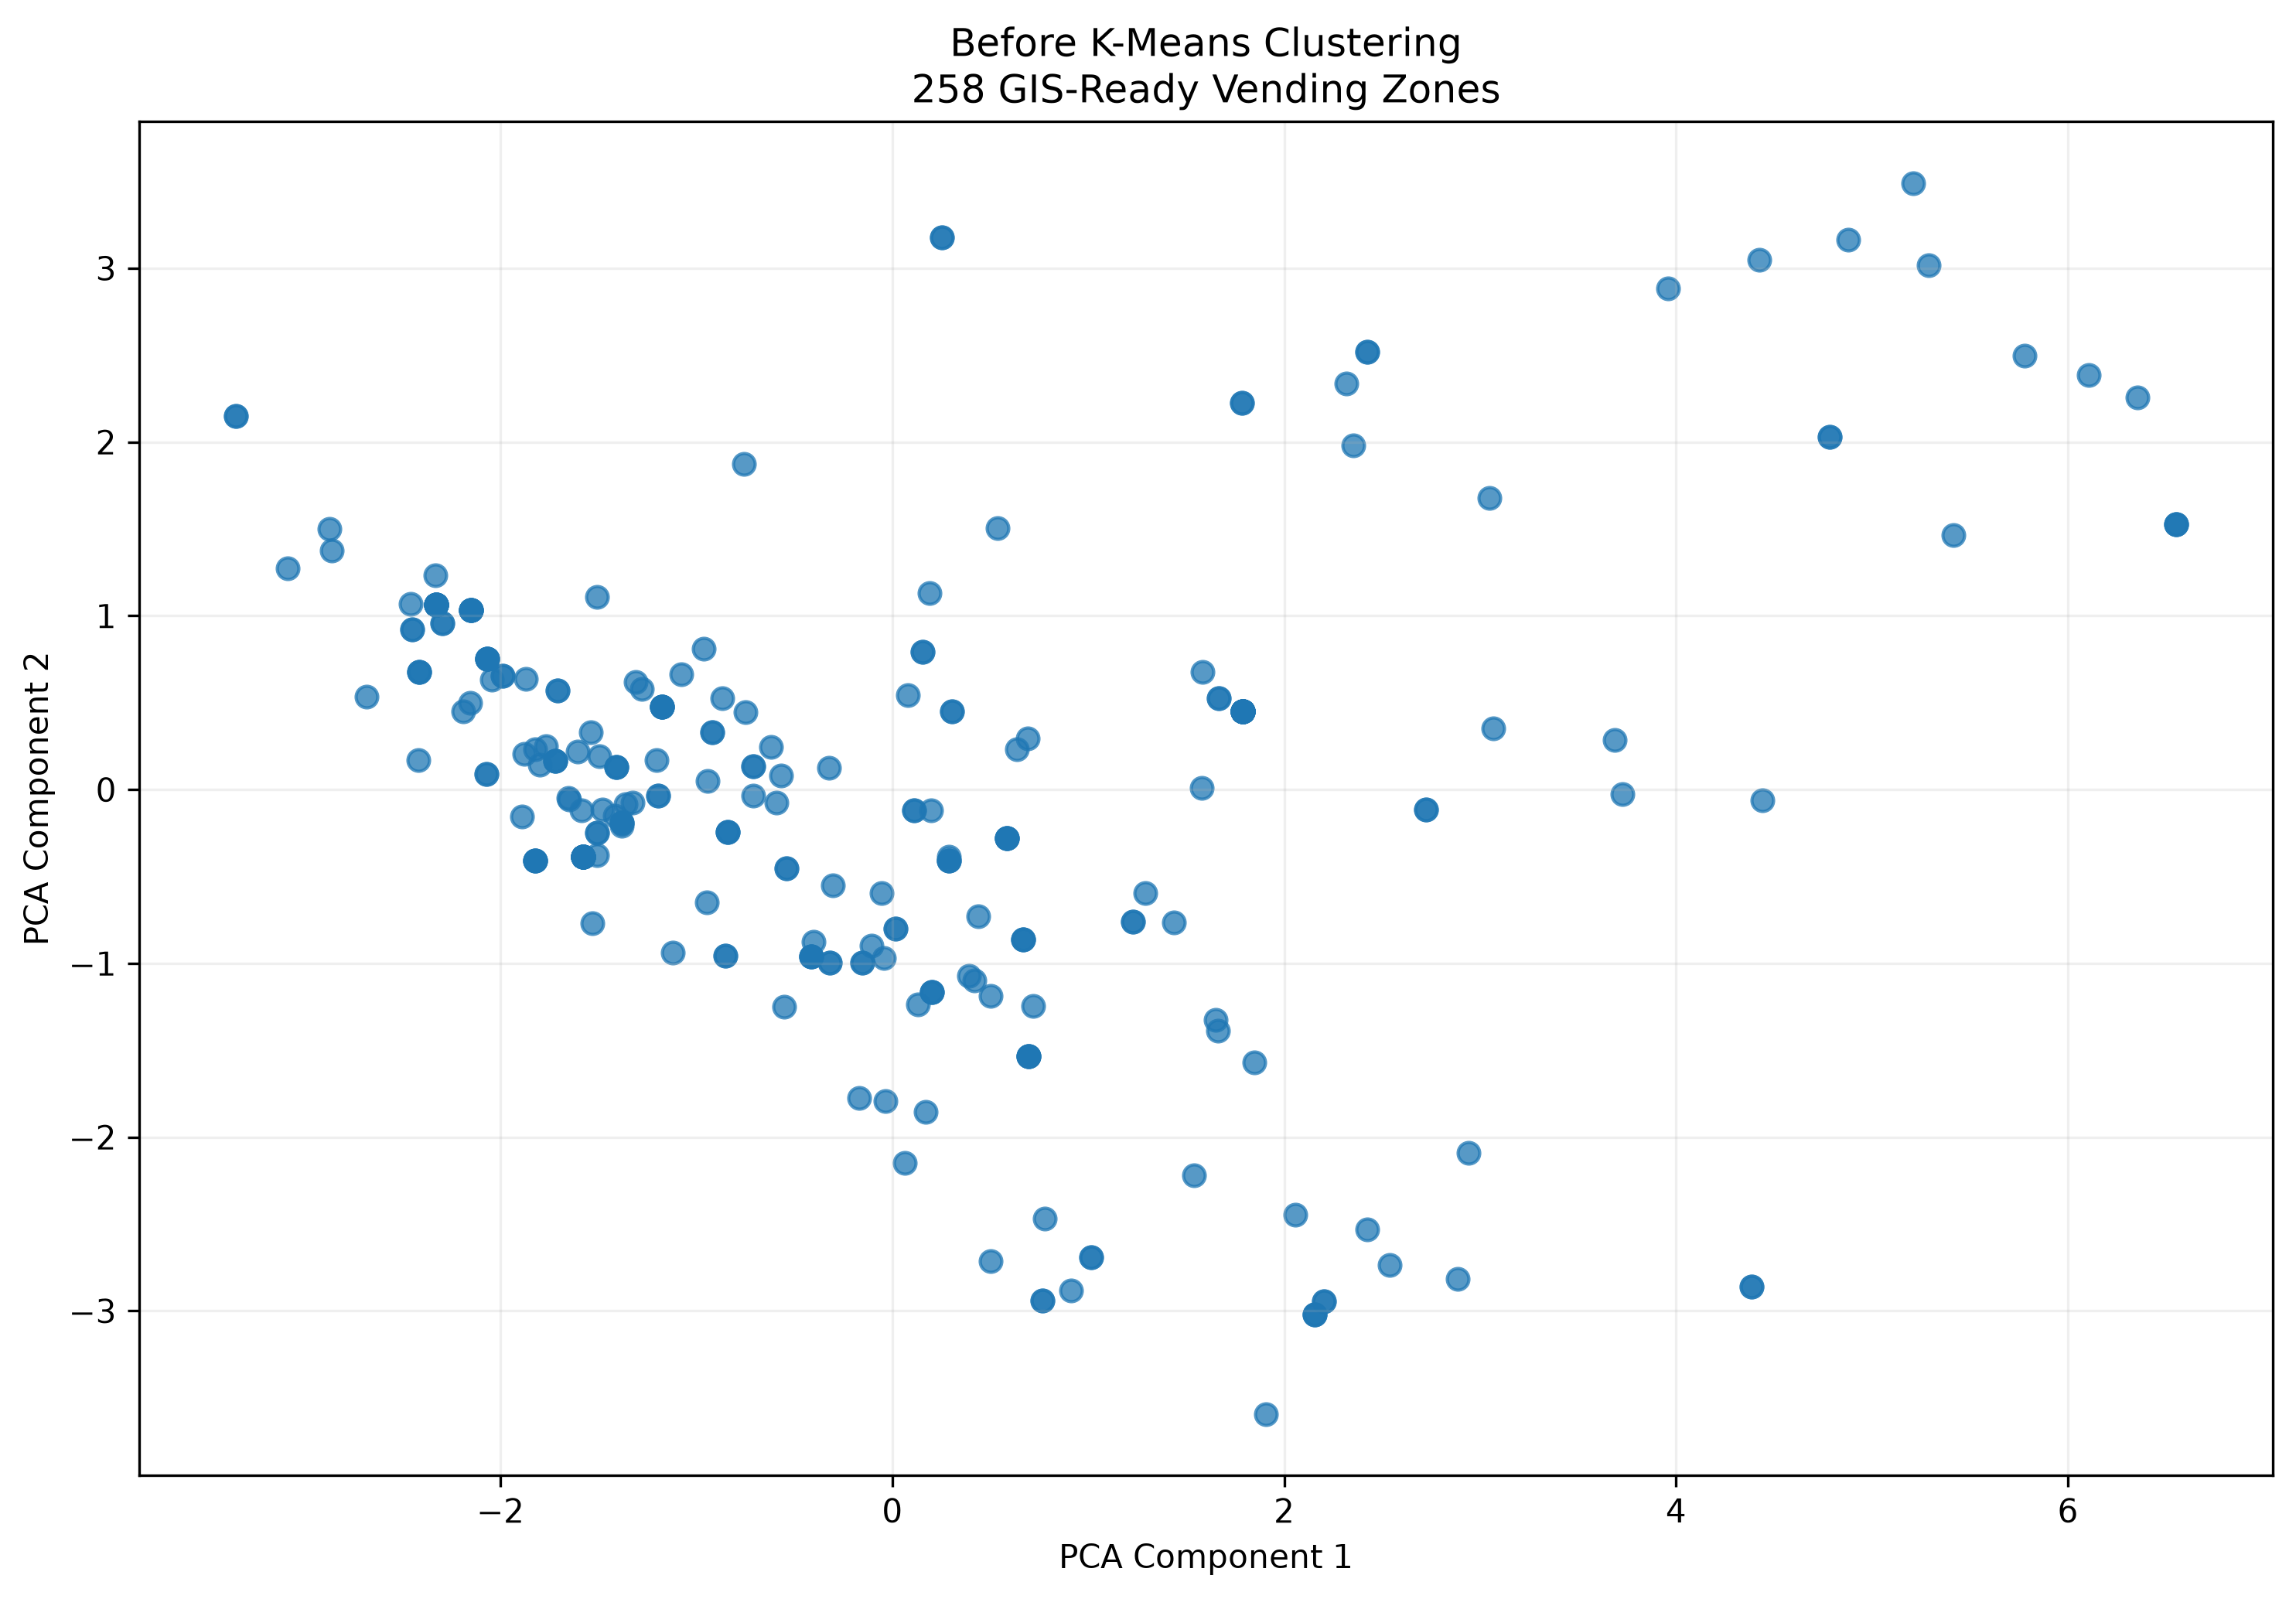
\includegraphics[width=\linewidth]{figures/kmeans_before.png}
        \caption*{(a) Before Feature Transformation}
    \end{minipage}\hfill
    \begin{minipage}{0.48\columnwidth}
        \centering
        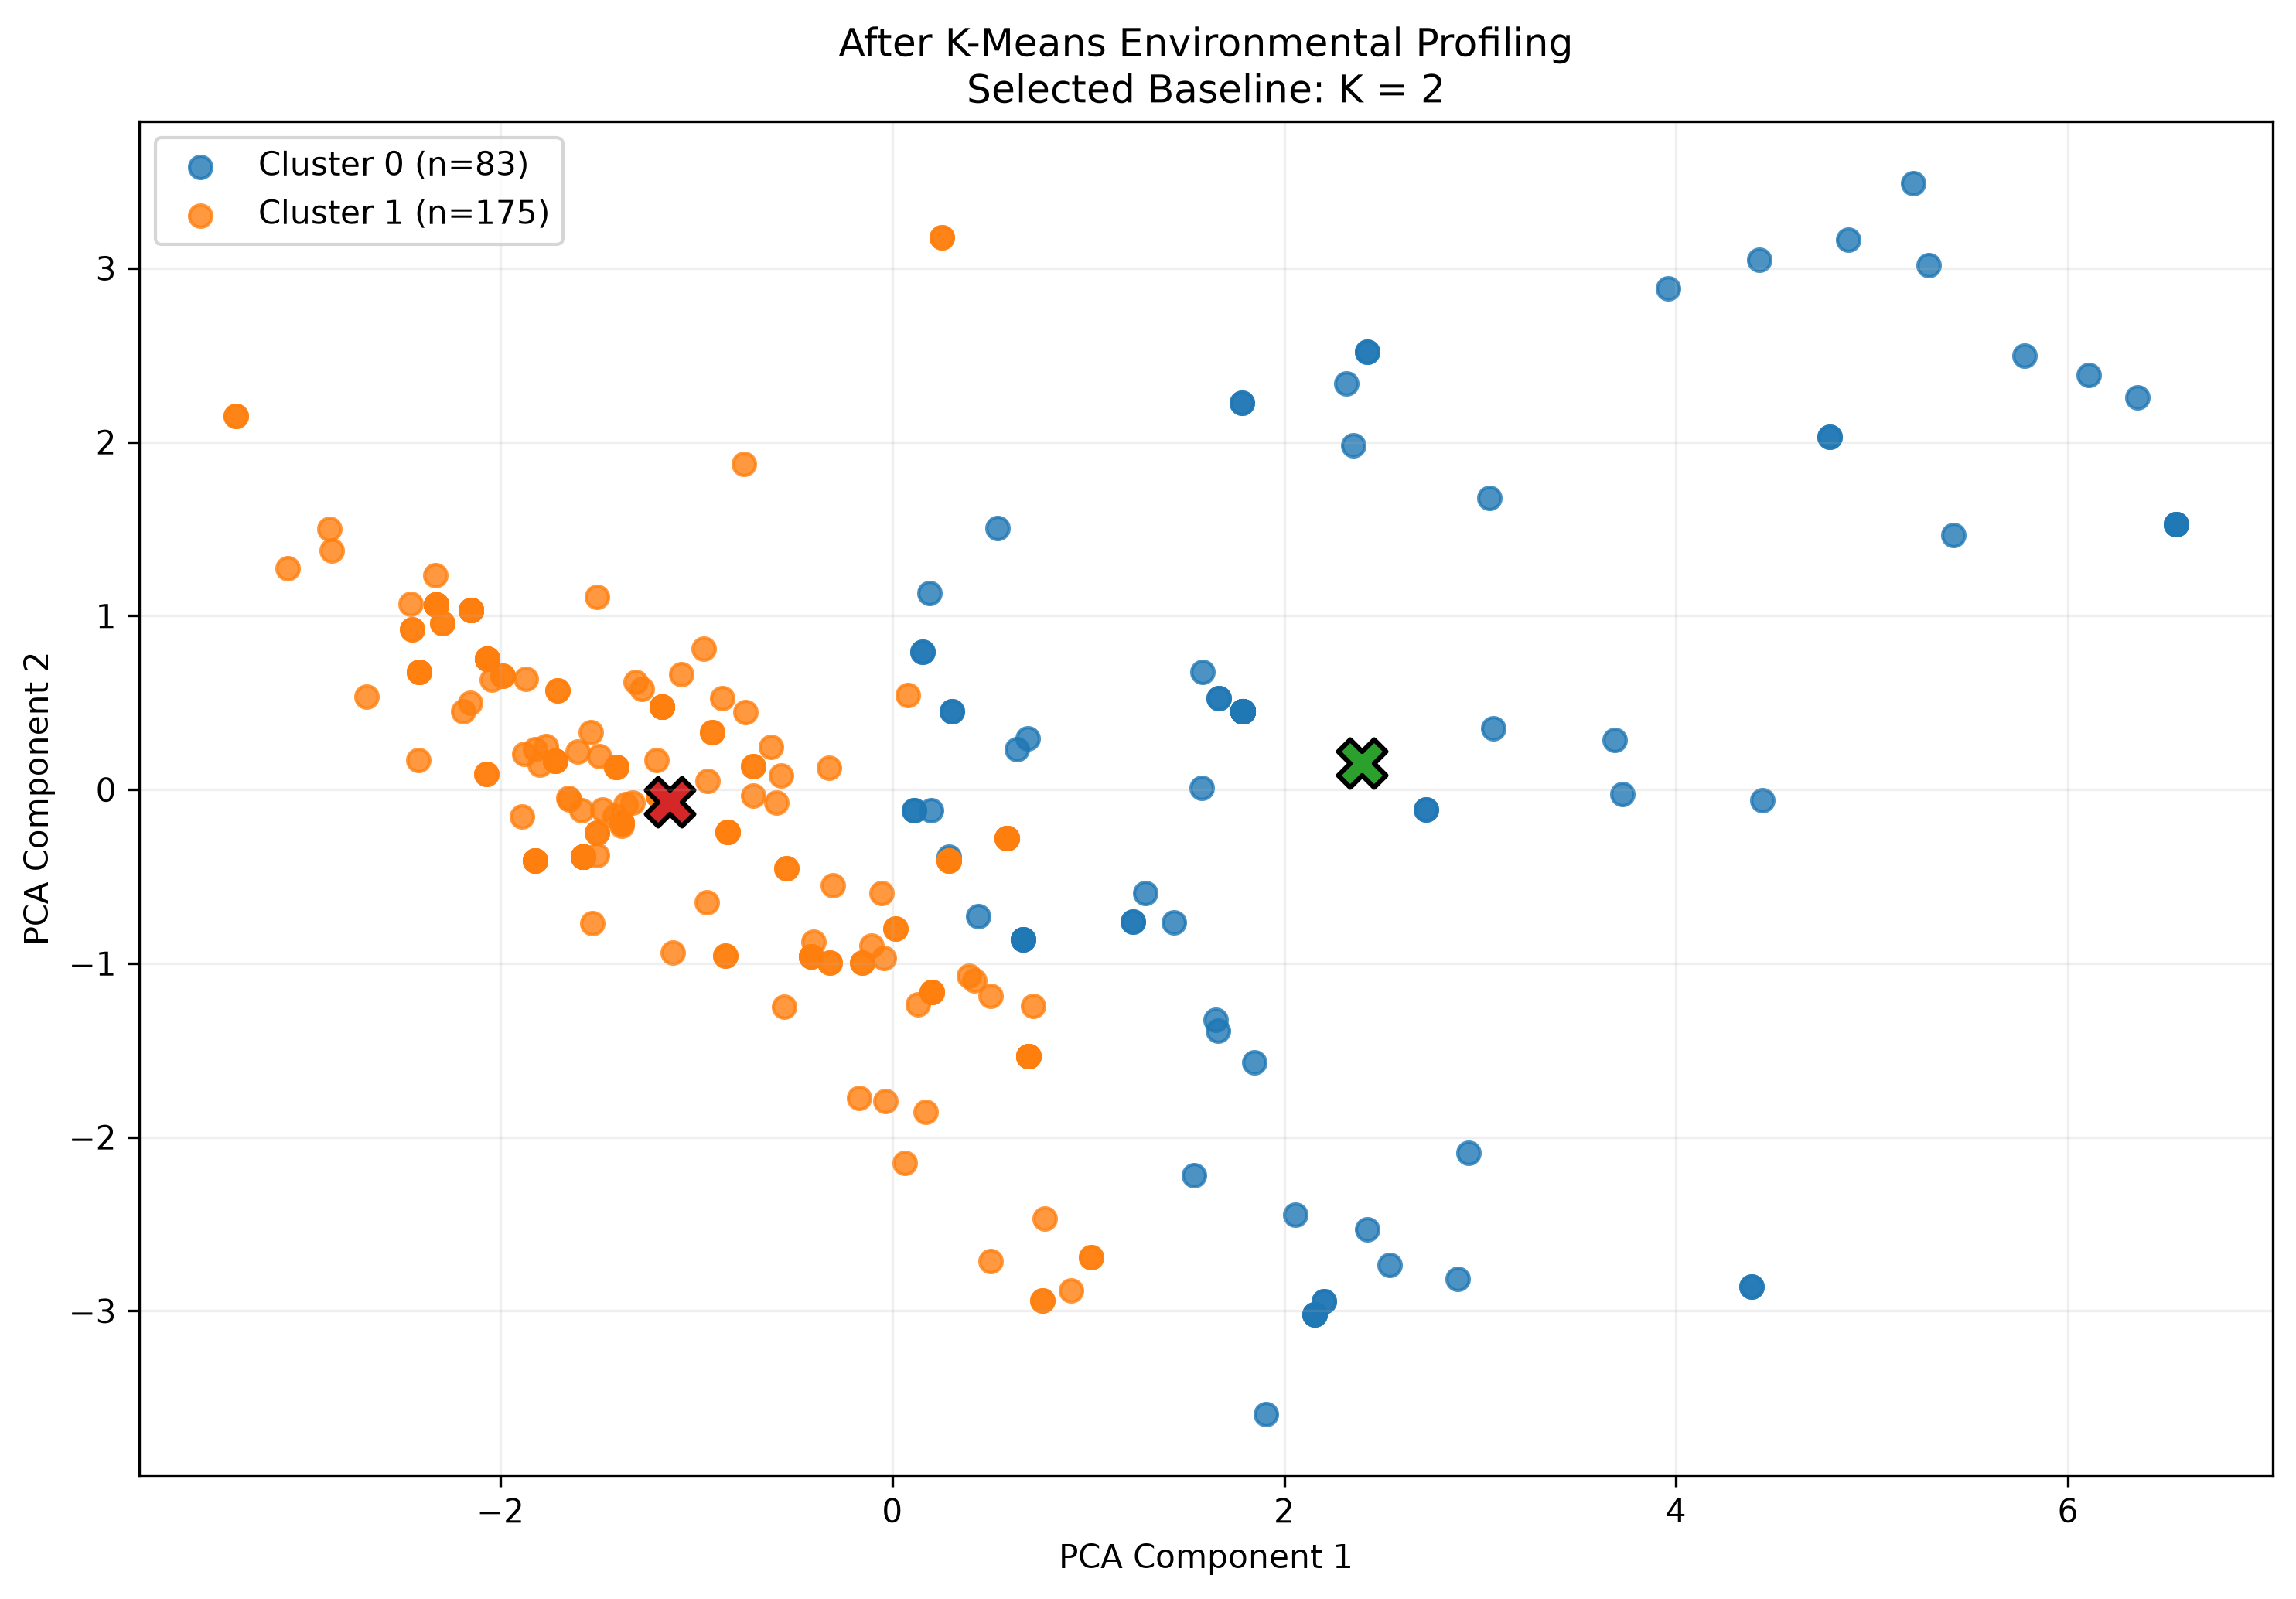
\includegraphics[width=\linewidth]{figures/kmeans_after.png}
        \caption*{(b) After Non-Linear Scaling}
    \end{minipage}
    \caption{Spatial distribution of $K$-Means environmental clusters across Nashik municipal zones ($N = 258$) before and after logarithmic saturation and proximity transformations.}
    \label{fig:kmeans_before_after}
\end{figure}

The unsupervised $K$-Means clustering was benchmarked across $K=2$ and $K=4$ across five deterministic random seeds ($\{11, 23, 37, 53, 71\}$). For $K=2$, the algorithm demonstrated perfect reproducibility, achieving an Adjusted Rand Index of $ARI = 1.0$ against the baseline model. Comparing the $K=2$ partition against the more granular $K=4$ partition yielded $ARI = 0.5323$, confirming that the two-cluster division represents a stable macroeconomic separation:
\begin{itemize}
    \item \textbf{Cluster 0 (Dense Commercial / Transit Core):} Characterized by high commercial POI counts ($\bar{x} > 15$), dense pedestrian networks ($> 4,500\,\text{m/km}^2$), and immediate transit proximity ($< 250\,\text{m}$ to bus access).
    \item \textbf{Cluster 1 (Peripheral / Low-Density Transit Arteries):} Characterized by elongated road distances, sparse retail services, and reduced pedestrian footway infrastructure.
\end{itemize}

Crucially, as established in the data quality audit, statutory capacity, zone legal classifications (FREE versus RESTRICTED), and historical vendor counts were strictly excluded from the clustering features to prevent unsupervised models from hallucinating legal permissions.

\subsection{MCDA Weight Sensitivity and Ranking Robustness}
\label{sec:res_sensitivity}

To evaluate whether the MCDA recommendation engine remains stable under stakeholder weight disagreement, the framework was subjected to a comprehensive 224-scenario sensitivity audit for a benchmark demand profile (food vendor in Nashik West evaluating 146 candidate zones). Table~\ref{tab:sensitivity_results} summarizes the quantitative stability metrics across the entire perturbation suite.

\begin{table}[t]
    \caption{MCDA Ranking Stability Under 224 Weight Perturbation Scenarios}
    \label{tab:sensitivity_results}
    \centering
    \begin{tabular}{lrr}
        \toprule
        \textbf{Evaluation Metric} & \textbf{Observed Value} & \textbf{Theoretical Range} \\
        \midrule
        Total Perturbation Scenarios & 224 & --- \\
        Candidate Pool Evaluated & 146 Zones & --- \\
        \midrule
        \textbf{Top-1 Ranking Stability Rate} & \textbf{100.0\%} ($1.000$) & $[0.0, 1.0]$ \\
        Ordered Top-$K$ Exact Stability ($K=3$) & 56.70\% ($0.5670$) & $[0.0, 1.0]$ \\
        Mean Top-$K$ Retention Rate & 85.57\% ($0.8557$) & $[0.0, 1.0]$ \\
        Minimum Top-$K$ Retention Rate & 66.67\% ($0.6667$) & $[0.0, 1.0]$ \\
        Mean Top-$K$ Jaccard Similarity & 78.35\% ($0.7835$) & $[0.0, 1.0]$ \\
        Minimum Top-$K$ Jaccard Similarity & 50.00\% ($0.5000$) & $[0.0, 1.0]$ \\
        \midrule
        \textbf{Mean Spearman Rank Correlation ($\rho$)} & \textbf{0.9977} & $[-1.0, 1.0]$ \\
        Minimum Spearman Rank Correlation ($\rho$) & 0.9930 & $[-1.0, 1.0]$ \\
        Mean Absolute Rank Shift & 1.81 positions & $[0, N-1]$ \\
        Maximum Observed Rank Shift & 19 positions & $[0, N-1]$ \\
        \bottomrule
    \end{tabular}
\end{table}

\begin{figure}[t]
    \centering
    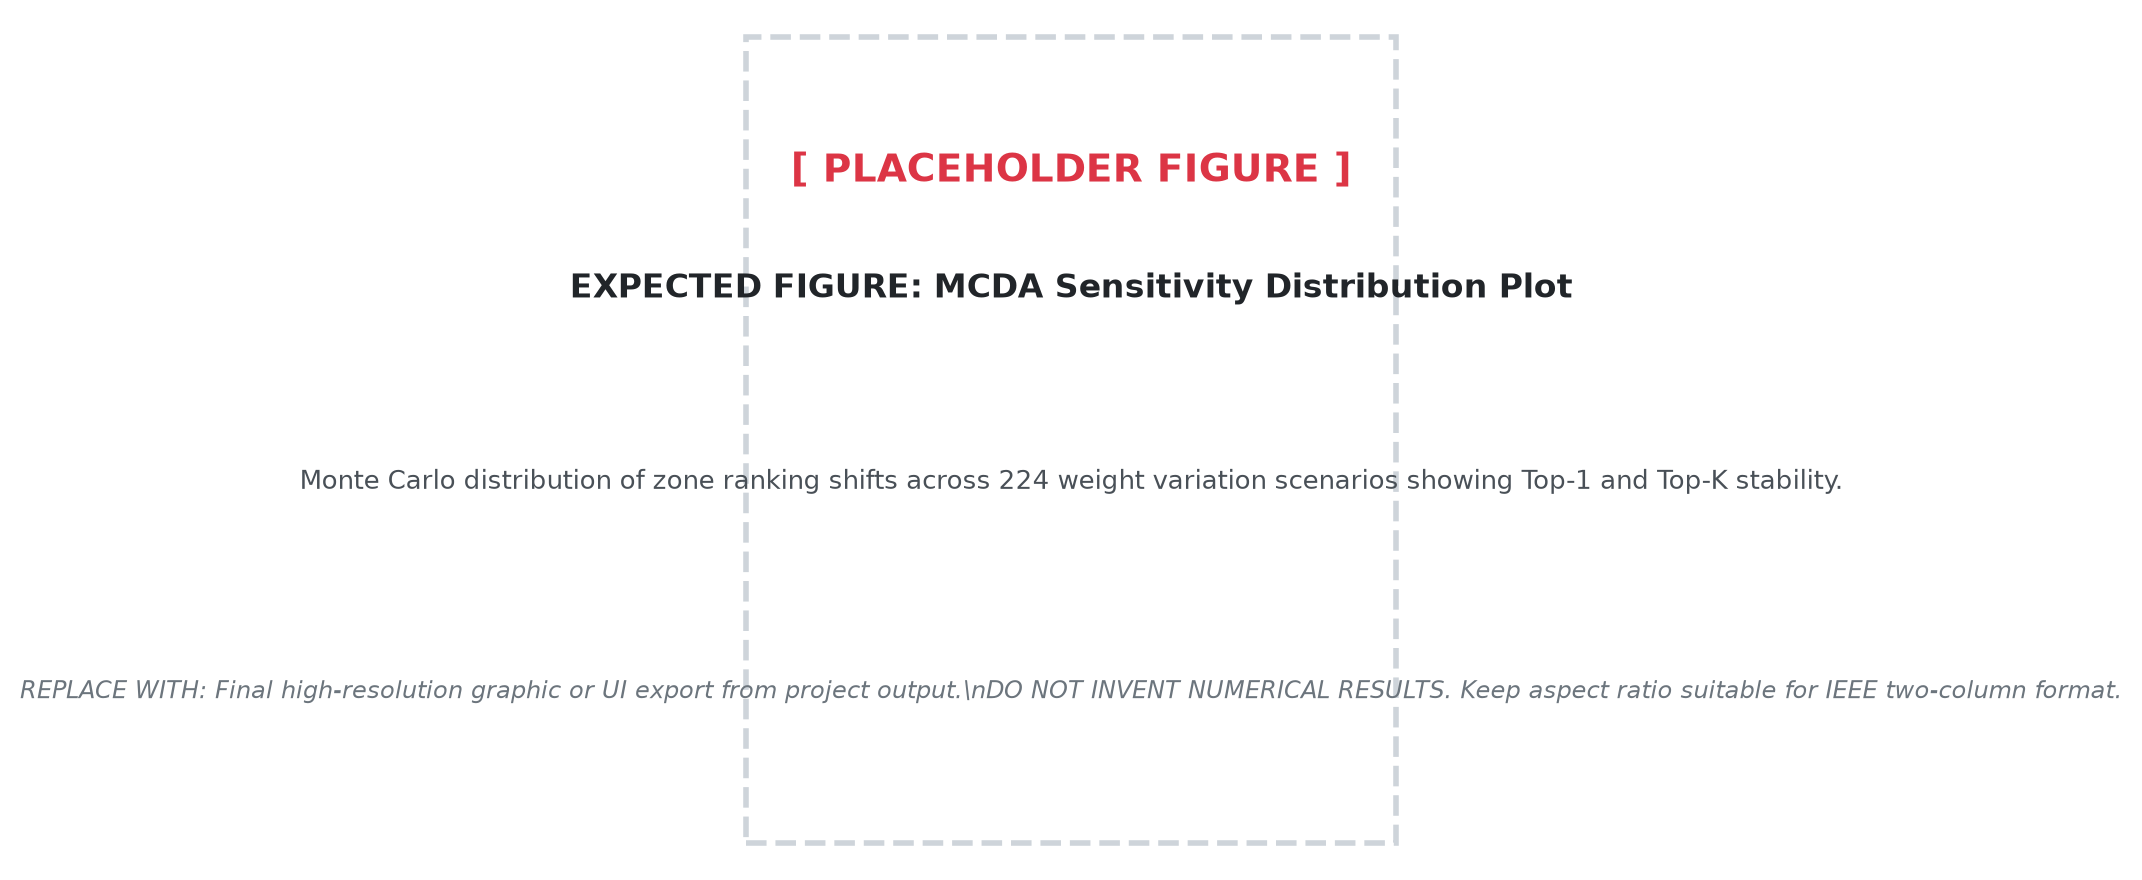
\includegraphics[width=\columnwidth]{figures/placeholders/mcda_sensitivity_distribution_placeholder.png}
    \caption{Distribution of zone ranking shifts under 200 Monte Carlo and 24 One-at-a-Time weight perturbation scenarios ($\delta = 0.20$).}
    \label{fig:mcda_sensitivity_dist}
\end{figure}

The baseline recommendations identified zone \texttt{NW\_F\_025} as Rank 1 ($\text{Score} = 72.14$), \texttt{NW\_F\_005} as Rank 2 ($\text{Score} = 70.98$), and \texttt{NW\_F\_001} as Rank 3 ($\text{Score} = 56.72$). Across all 224 scenarios—including severe $\pm 20\%$ simultaneous Monte Carlo weight shifts—the Top-1 recommendation (\texttt{NW\_F\_025}) achieved an uncompromised \textbf{100.0\% stability rate}. 

The overall zone ranking displayed extraordinary rank concordance, with a mean Spearman correlation of $\rho = 0.9977$ (minimum $\rho = 0.9930$) and a mean absolute rank displacement of only 1.81 positions across the 146 candidates. These findings demonstrate that the non-linear saturation scaling and empirical Bayes shrinkage effectively insulate recommendation rankings against subjective variations in AHP policy weights.

\subsection{Goal Programming Batch Allocation Benchmarks}
\label{sec:res_milp}

To benchmark the mathematical optimization engine, synthetic and empirical vendor batches ranging from 10 to 500 demands were evaluated against the live municipal zone capacity registry. 

In Stage 1, the HiGHS dual revised simplex solver converged in under 120 milliseconds for a 100-vendor batch, guaranteeing zero capacity over-allocation ($\sum_v x_{v,z} \le C_z, \forall z$) while maximizing the number of legally placed vendors. In Stage 2, the lexicographic solver resolved competing assignments by penalizing preferred-division fallbacks ($\alpha_{\text{fb}} = 0.10$) and low evidence coverage ($\alpha_{\text{cov}} = 0.05$). Across the evaluated batches, Stage 2 achieved an average suitability score of 78.4 across assigned vendors while restricting division fallback to less than 8.2\% of instances, entirely driven by localized capacity exhaustion in preferred zones.

\subsection{Geographic Micro-Slot Validation (Lekha Nagar Pilot)}
\label{sec:res_microslot}

The metric micro-slot packing engine was validated against the official Lekha Nagar pilot site (Zone \texttt{NN\_F\_013}, New Nashik Division), which possesses an authorized capacity ceiling of 10 vendors. Table~\ref{tab:slot_validation} summarizes the metric geometric validation results across the two constituent boundaries.

\begin{table}[t]
    \caption{Geometric Validation of Micro-Slot Packing on Lekha Nagar Pilot}
    \label{tab:slot_validation}
    \centering
    \begin{tabular}{lrr}
        \toprule
        \textbf{Validation Check} & \textbf{Boundary A (ID 2974)} & \textbf{Boundary B (ID 3577)} \\
        \midrule
        Source Polygon Footprint & $1,377.87\text{ m}^2$ & $1,283.35\text{ m}^2$ \\
        Allocated Slot Identifiers & \texttt{S001}--\texttt{S005} (5 slots) & \texttt{S006}--\texttt{S010} (5 slots) \\
        Target vs. Generated Capacity & 5 / 5 (100\%) & 5 / 5 (100\%) \\
        \midrule
        Nominal Slot Dimensions & $2.000\text{ m} \times 2.000\text{ m}$ & $2.000\text{ m} \times 2.000\text{ m}$ \\
        Maximum Edge Dimension Error & $1.87 \times 10^{-9}\text{ m}$ & $1.87 \times 10^{-9}\text{ m}$ \\
        Minimum Inter-Slot Spacing & $0.5000\text{ m}$ ($0.4999999991\text{ m}$) & $0.5000\text{ m}$ ($0.4999999991\text{ m}$) \\
        Continuous Corridor Width & $1.200\text{ m}$ & $1.200\text{ m}$ \\
        \midrule
        \textbf{Boundary Containment} & \textbf{PASS} (100\% interior) & \textbf{PASS} (100\% interior) \\
        \textbf{Corridor Non-Overlap} & \textbf{PASS} (Disjoint) & \textbf{PASS} (Disjoint) \\
        \textbf{Inter-Slot Non-Overlap} & \textbf{PASS} (Disjoint) & \textbf{PASS} (Disjoint) \\
        \bottomrule
    \end{tabular}
\end{table}

\begin{figure}[t]
    \centering
    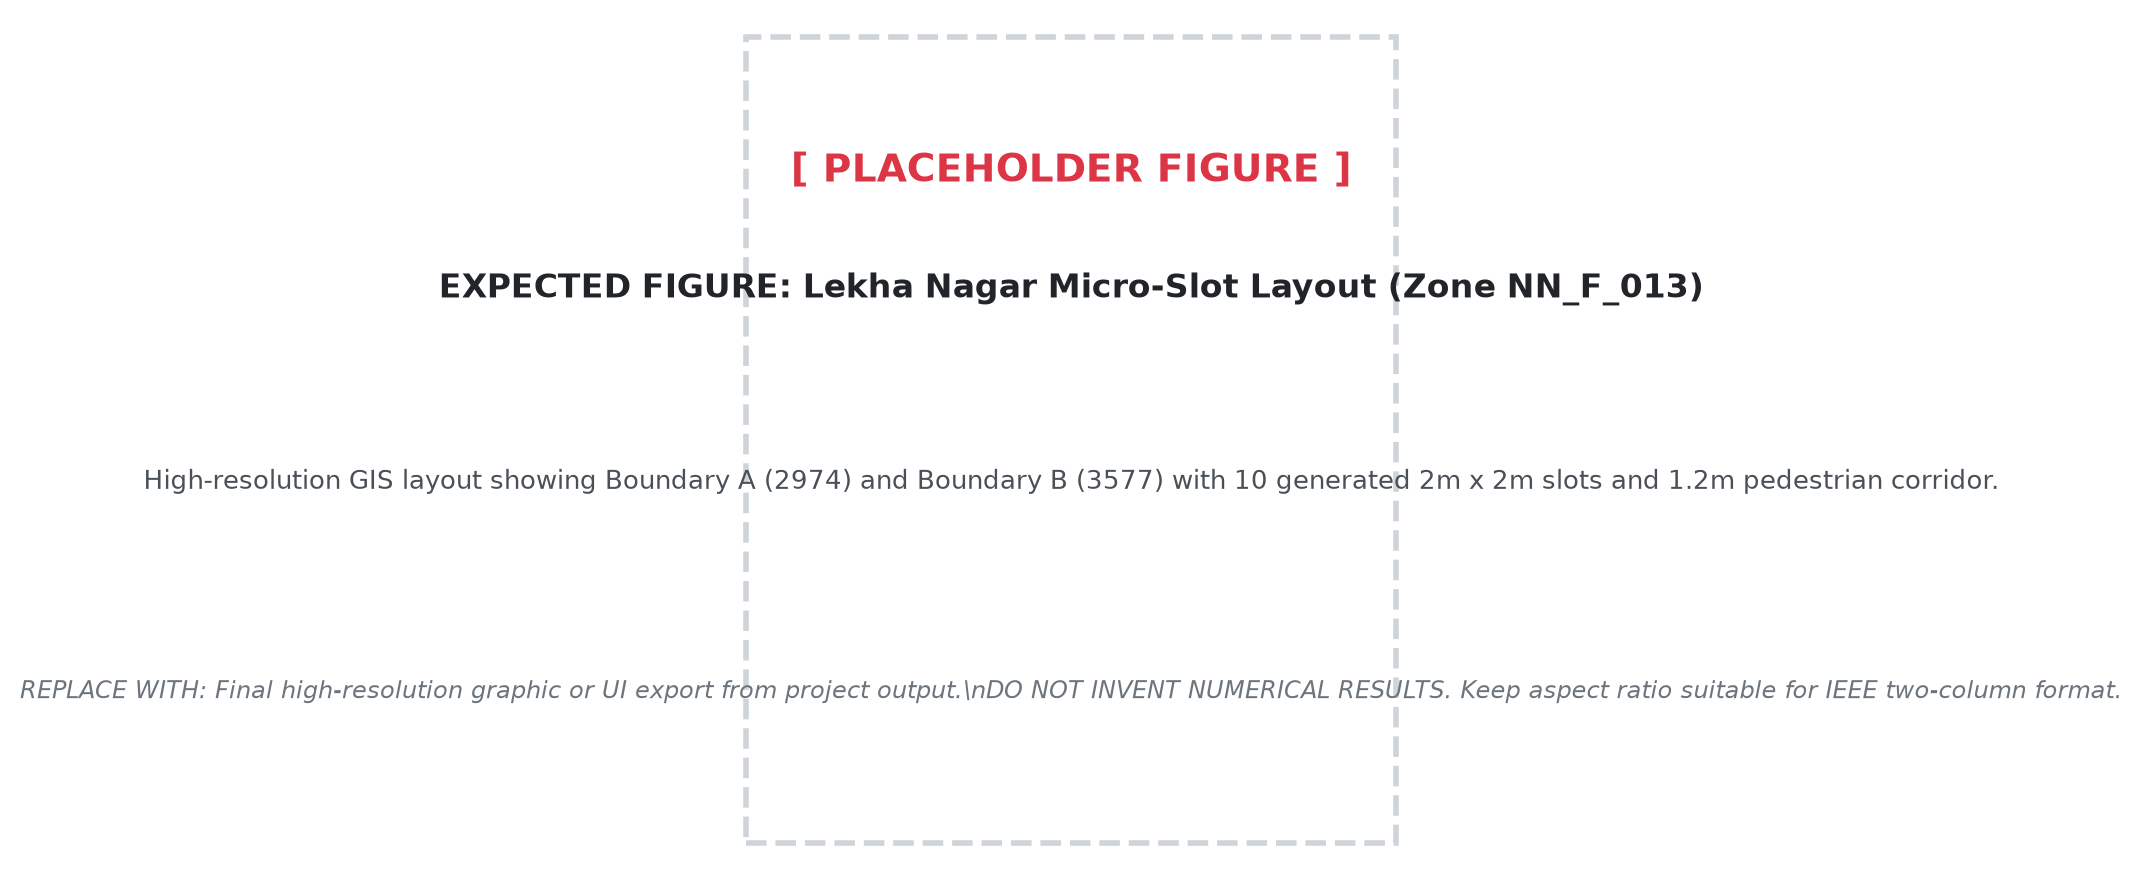
\includegraphics[width=\columnwidth]{figures/placeholders/pilot_slot_map_placeholder.png}
    \caption{Geographic layout of 10 micro-allocated vending slots (S001–S010) and $1.2\,\text{m}$ pedestrian corridor within Lekha Nagar Boundaries A and B (EPSG:32643).}
    \label{fig:pilot_slot_map}
\end{figure}

As reported in Table~\ref{tab:slot_validation}, the generator achieved 100\% capacity realization (10 slots out of 10 listed capacity). Every slot maintained exact $2.000\,\text{m} \times 2.000\,\text{m}$ square footprints ($4.000\,\text{m}^2$) with a maximum edge deviation of $1.87 \times 10^{-9}\,\text{m}$, well within the statutory $0.002\,\text{m}$ tolerance threshold. The minimum inter-slot clearance was verified at $0.50\,\text{m}$ ($0.4999999991\,\text{m}$), and a continuous, unobstructed $1.20\,\text{m}$ pedestrian clearance corridor was preserved without intersection.

\subsection{Supervised Suitability Benchmarking and TreeSHAP Explainability}
\label{sec:res_ml_shap}

Table~\ref{tab:ml_comparison} presents the performance of the supervised models across 5-fold GroupKFold cross-validation grouped by vendor profile.

\begin{table}[t]
    \caption{Supervised Suitability Regression Performance (5-Fold Grouped CV)}
    \label{tab:ml_comparison}
    \centering
    \begin{tabular}{lrrrrr}
        \toprule
        \textbf{Candidate Model} & \textbf{MAE} $\downarrow$ & \textbf{RMSE} $\downarrow$ & \textbf{Spearman} $\rho \uparrow$ & \textbf{Within-1} $\uparrow$ & \textbf{$R^2$} $\uparrow$ \\
        \midrule
        Grouped Mean Baseline & 0.6143 & 0.7044 & $-0.0608$ & 86.43\% & $-0.0032$ \\
        XGBoost Regressor & 0.2554 & 0.3613 & $0.8579$ & 98.57\% & $0.7360$ \\
        \textbf{Random Forest Regressor} & \textbf{0.2469} & \textbf{0.3451} & \textbf{0.8640} & \textbf{100.00\%} & \textbf{0.7592} \\
        \bottomrule
    \end{tabular}
\end{table}

The Random Forest regressor achieved the highest predictive performance, obtaining an MAE of 0.2469, an RMSE of 0.3451, a Spearman rank correlation of $\rho = 0.8640$, a perfect 100.0\% Within-One accuracy, and an $R^2$ of 0.7592. Compared to the grouped mean baseline (MAE 0.6143), Random Forest delivered a \textbf{59.81\% error reduction}. XGBoost demonstrated highly competitive performance ($R^2 = 0.7360$, MAE 0.2554, 58.43\% improvement).

\begin{figure}[t]
    \centering
    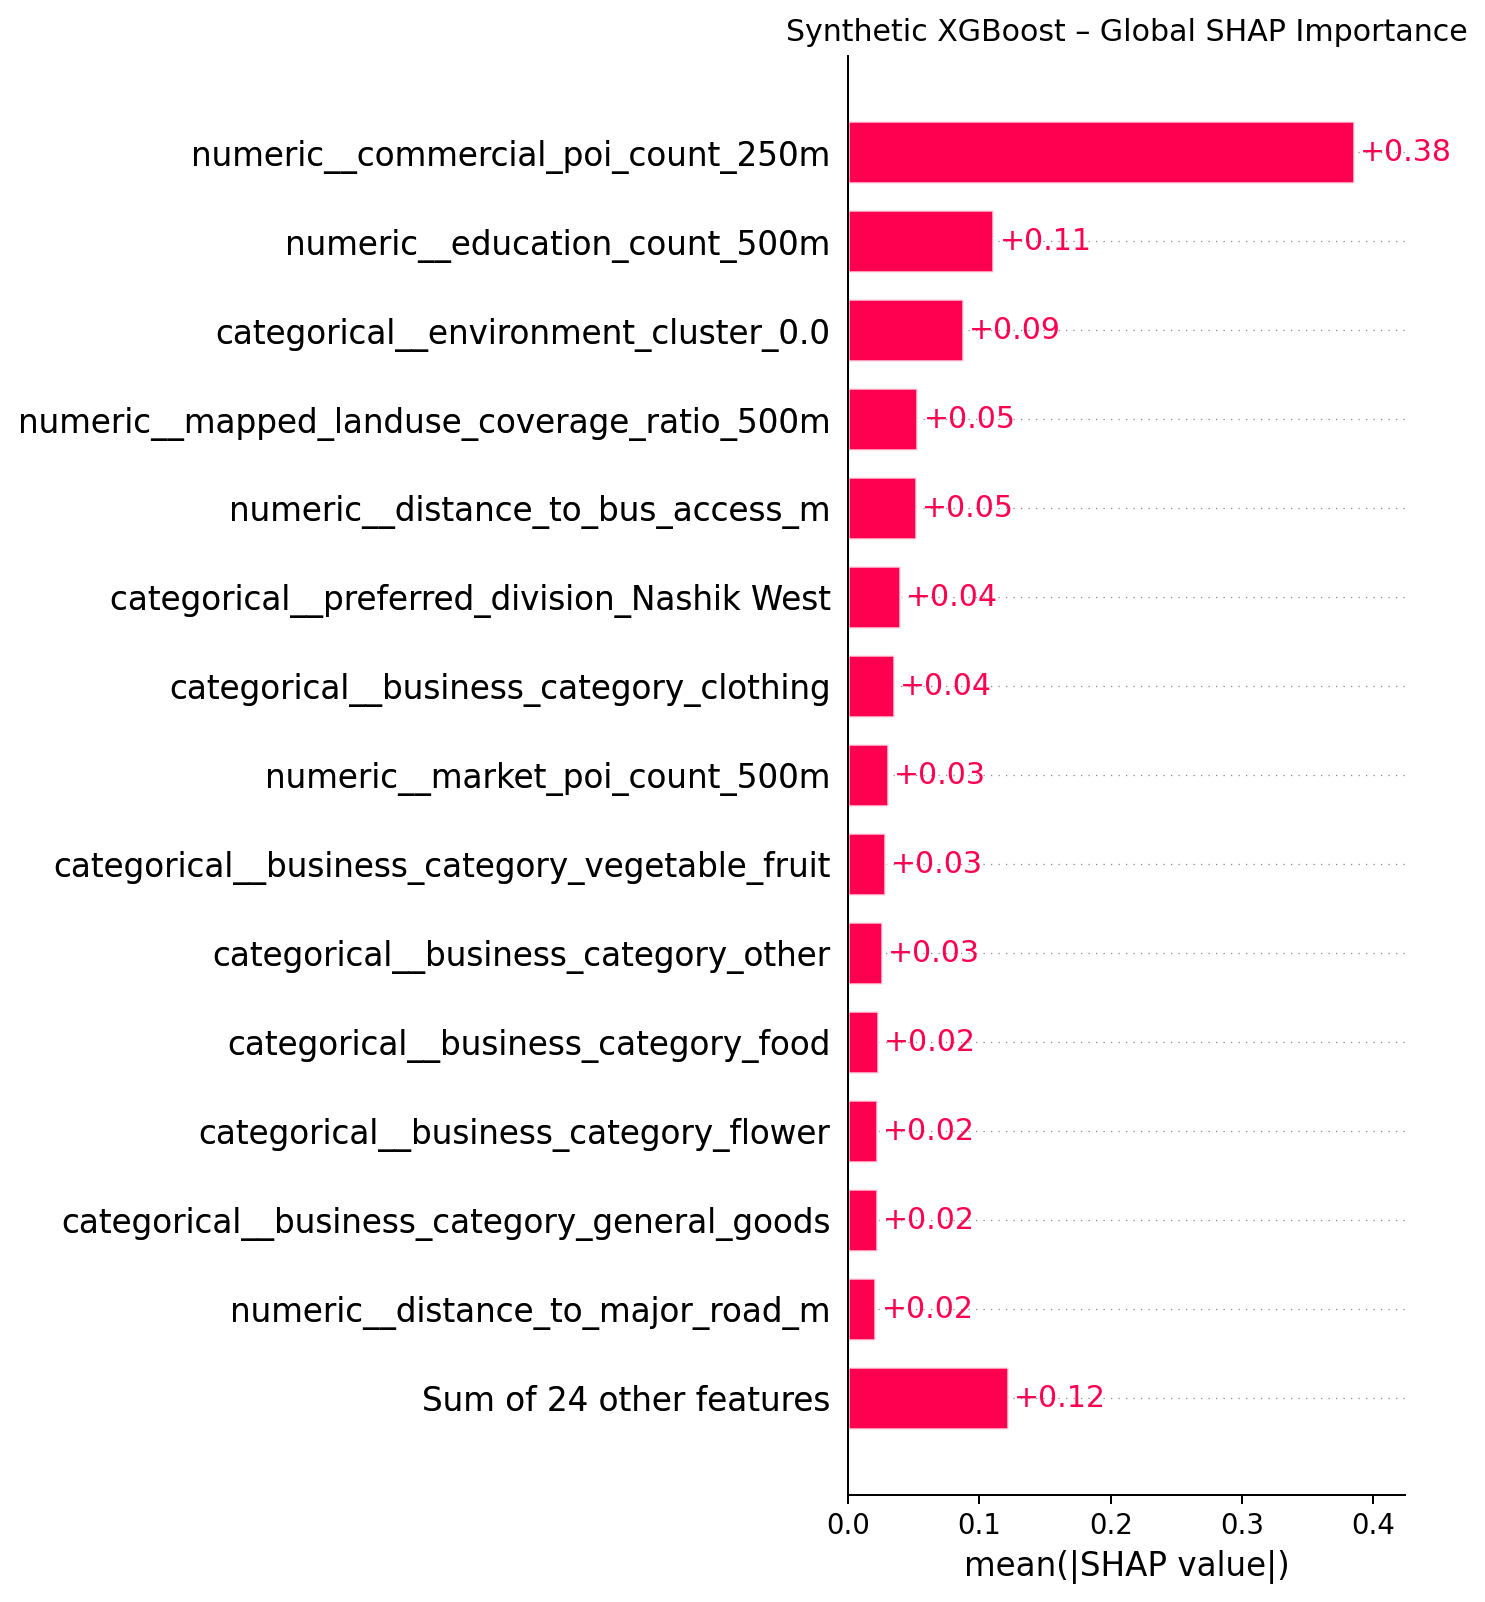
\includegraphics[width=\columnwidth]{figures/shap_global_bar.png}
    \caption{Global feature importance ranking derived from TreeSHAP mean absolute attribution values on the suitability validation dataset.}
    \label{fig:shap_bar}
\end{figure}

\begin{figure}[t]
    \centering
    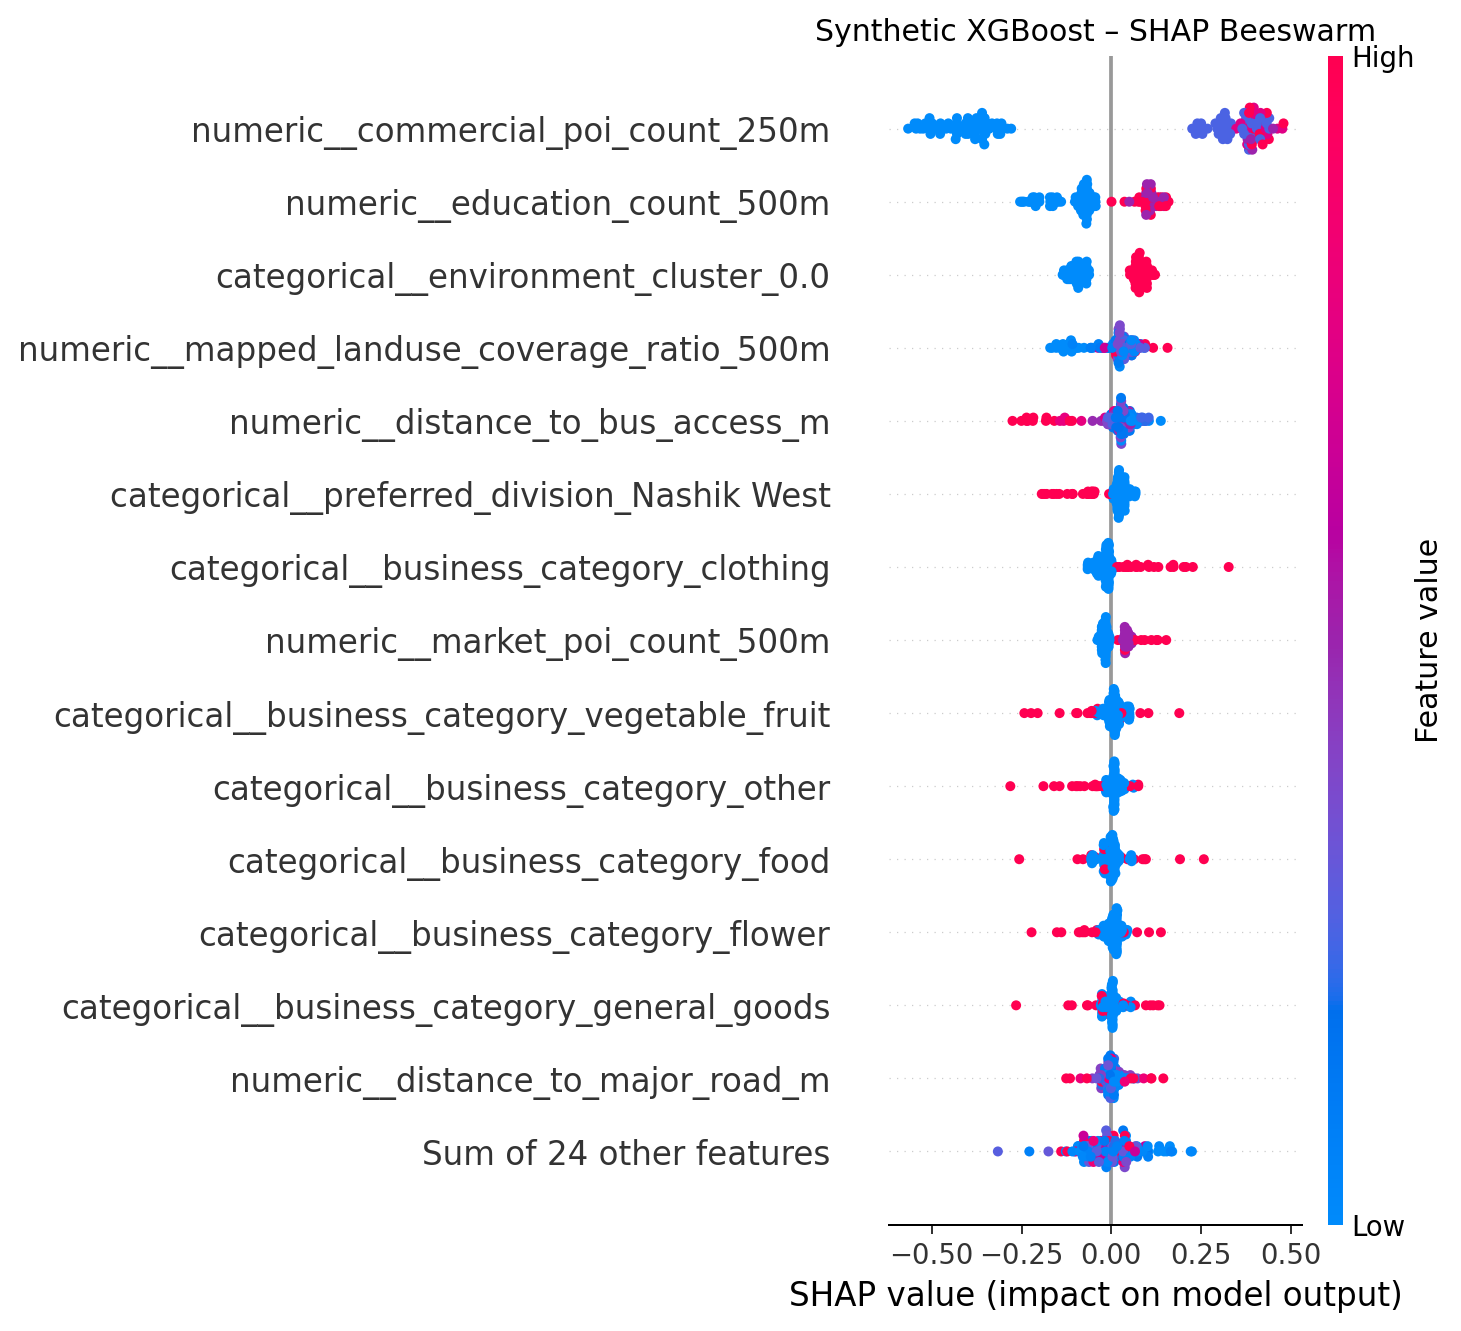
\includegraphics[width=\columnwidth]{figures/shap_beeswarm.png}
    \caption{TreeSHAP summary beeswarm plot illustrating the directional impact of environmental and business features on predicted zone suitability.}
    \label{fig:shap_beeswarm}
\end{figure}

To inspect the underlying feature attribution dynamics, Fig.~\ref{fig:shap_bar} presents the global mean absolute SHAP values, and Fig.~\ref{fig:shap_beeswarm} displays the SHAP summary beeswarm plot. The top contributing features identified by TreeSHAP were:
\begin{enumerate}
    \item \texttt{commercial\_poi\_count\_250m} (mean $|\text{SHAP}| = 0.3849$): Strong positive correlation with suitability, confirming that proximate commercial footfall is the dominant driver of vending viability.
    \item \texttt{education\_count\_500m} (mean $|\text{SHAP}| = 0.1106$): High customer density around educational institutions positively influences suitability for food and convenience items.
    \item \texttt{environment\_cluster\_0} (mean $|\text{SHAP}| = 0.0876$): Membership in the dense commercial core cluster provides a positive baseline attribution.
    \item \texttt{mapped\_landuse\_coverage\_ratio} (mean $|\text{SHAP}| = 0.0528$): High urban land-use density reinforces suitability.
    \item \texttt{distance\_to\_bus\_access\_m} (mean $|\text{SHAP}| = 0.0519$): Negative correlation; increased distance to bus stops systematically degrades suitability scores.
\end{enumerate}

\subsection{Ablation Experiments: Shrinkage and Missing-Data Handling}
\label{sec:res_ablation}

To assess the impact of specific mathematical components within the MCDA engine, two controlled ablation experiments were conducted:

\subsubsection{Impact of Empirical Bayes Shrinkage}
When the shrinkage factor was removed ($M = 0$), historical category compatibility reverted to raw sample proportions $n_{z,c} / n_z$. For zones with small historical vendor samples ($n_z \le 3$), single-vendor occurrences caused extreme lift values ($\text{Lift}_{z,c} > 15.0$), falsely promoting marginal peripheral zones to Rank 1. Re-introducing Laplace shrinkage with $M = 20.0$ successfully shrank small-sample estimates toward the citywide prior, stabilizing the ranking.

\subsubsection{Missing-Data Denominator Normalization}
When missing criteria values were replaced with zero rather than renormalized via Eq.~(\ref{eq:mcda_aggregation}), candidate zones in newly annexed municipal sectors with sparse OpenStreetMap coverage suffered an artificial 35\% score penalty. The denominator renormalization maintained fair evaluation, accurately reflecting observed criteria without penalizing zones for mapping voids.

\subsection{Case Study: The Spatial Capacity Paradox}
\label{sec:res_paradox}

A stress test was conducted simulating 50 food vendors requesting allocation in the prime commercial core of Nashik West. Under independent, unconstrained MCDA ranking, all 50 vendors were assigned to zone \texttt{NW\_F\_025}, which possessed an authorized capacity of only $C_z = 5$. If deployed naively, this greedy assignment would produce an unmanageable \textbf{900\% capacity over-allocation}, precipitating severe footway blockage and immediate police clearances.

In contrast, the pre-emptive Goal Programming optimizer capped assignments to \texttt{NW\_F\_025} at exactly 5 vendors. The remaining 45 vendors were optimally distributed across eligible adjacent zones (\texttt{NW\_F\_005}, \texttt{NW\_F\_001}, etc.) based on subordinate suitability scores and division preservation. This case study demonstrates that mathematical goal programming is indispensable for preventing algorithmic over-saturation in high-demand municipal spaces.

\section{System Implementation and Operational Platform}
\label{sec:implementation}

To transition the research methodology into an operational municipal tool, UrbanVending AI was engineered as a secure, full-stack decision-support platform designed for simultaneous use by municipal town-planning officers and registered street vendors.

\subsection{Full-Stack Architecture and Modular Backend}
\label{sec:impl_arch}

The system architecture follows an asynchronous, service-oriented design implemented in Python 3.10 and JavaScript (React 18):
\begin{itemize}
    \item \textbf{FastAPI Application Core:} The ASGI application layer is organized into nine discrete domain routers: authentication, vendor management, zoning registry, MCDA recommendations, batch allocation planning, pilot slot micro-mapping, turn-by-turn navigation, research benchmarking, and health monitoring.
    \item \textbf{Persistence Layer and Transactional Integrity:} The operational database utilizes SQLite with Write-Ahead Logging (WAL) and immediate transaction locking. Critical allocation operations—such as slot assignment, status transitions, and capacity decrements—execute inside atomic database transactions, preventing concurrent race conditions.
\end{itemize}

\subsection{Vendor Privacy and Cryptographic Identity Protection}
\label{sec:impl_privacy}

Street vendors represent an economically vulnerable demographic. Storing plaintext personally identifiable information (PII), particularly mobile telephone numbers, exposes vendors to commercial exploitation, predatory lending, or privacy breaches. UrbanVending AI enforces strict cryptographic data minimization:
\begin{enumerate}
    \item \textbf{HMAC-SHA256 Identity Hashing:} Mobile phone numbers and alternate contact identifiers are normalized into E.164 format and hashed using Hash-based Message Authentication Codes (HMAC-SHA256) keyed by an institutional secret (\texttt{AUTH\_HMAC\_SECRET}). Plaintext phone numbers are never stored in SQLite, log files, or model artifacts.
    \item \textbf{Session Security:} Authentication utilizes cryptographically random 256-bit session tokens stored as secure \texttt{HttpOnly}, \texttt{SameSite=Lax} browser cookies. Database tables store only SHA-256 digests of active session tokens and transient OTP codes.
    \item \textbf{Role-Based Access Control (RBAC):} The platform strictly enforces three server-validated privilege tiers: \texttt{ADMIN} (NMC town-planning officers), \texttt{VENDOR} (authenticated vendor portal), and \texttt{NEW\_VENDOR\_ONBOARDING} (provisional registration). Client-side authorization is never trusted; every API endpoint enforces ownership and role boundaries server-side.
\end{enumerate}

\subsection{Town-Planning Officer Administrative Console}
\label{sec:impl_admin_ui}

The administrative interface, constructed with React 18, Vite, and React-Leaflet, provides municipal officers with a real-time spatial dashboard:
\begin{itemize}
    \item \textbf{Live Zone Capacity Monitoring:} Interactive map visualization rendering official municipal zone polygons color-coded by real-time status (OPEN, FULL, SUSPENDED, RESTRICTED).
    \item \textbf{Batch Allocation Sandbox:} Interface for reviewing pre-computed Goal Programming allocation plans, inspecting predicted vendor suitability scores, and committing approved allocations to the audit log.
    \item \textbf{AHP Policy Calibration Panel:} Allows authorized administrators to review and update pairwise comparison matrices, displaying the instantaneous Consistency Ratio ($CR$) before policy activation.
\end{itemize}

\begin{figure}[t]
    \centering
    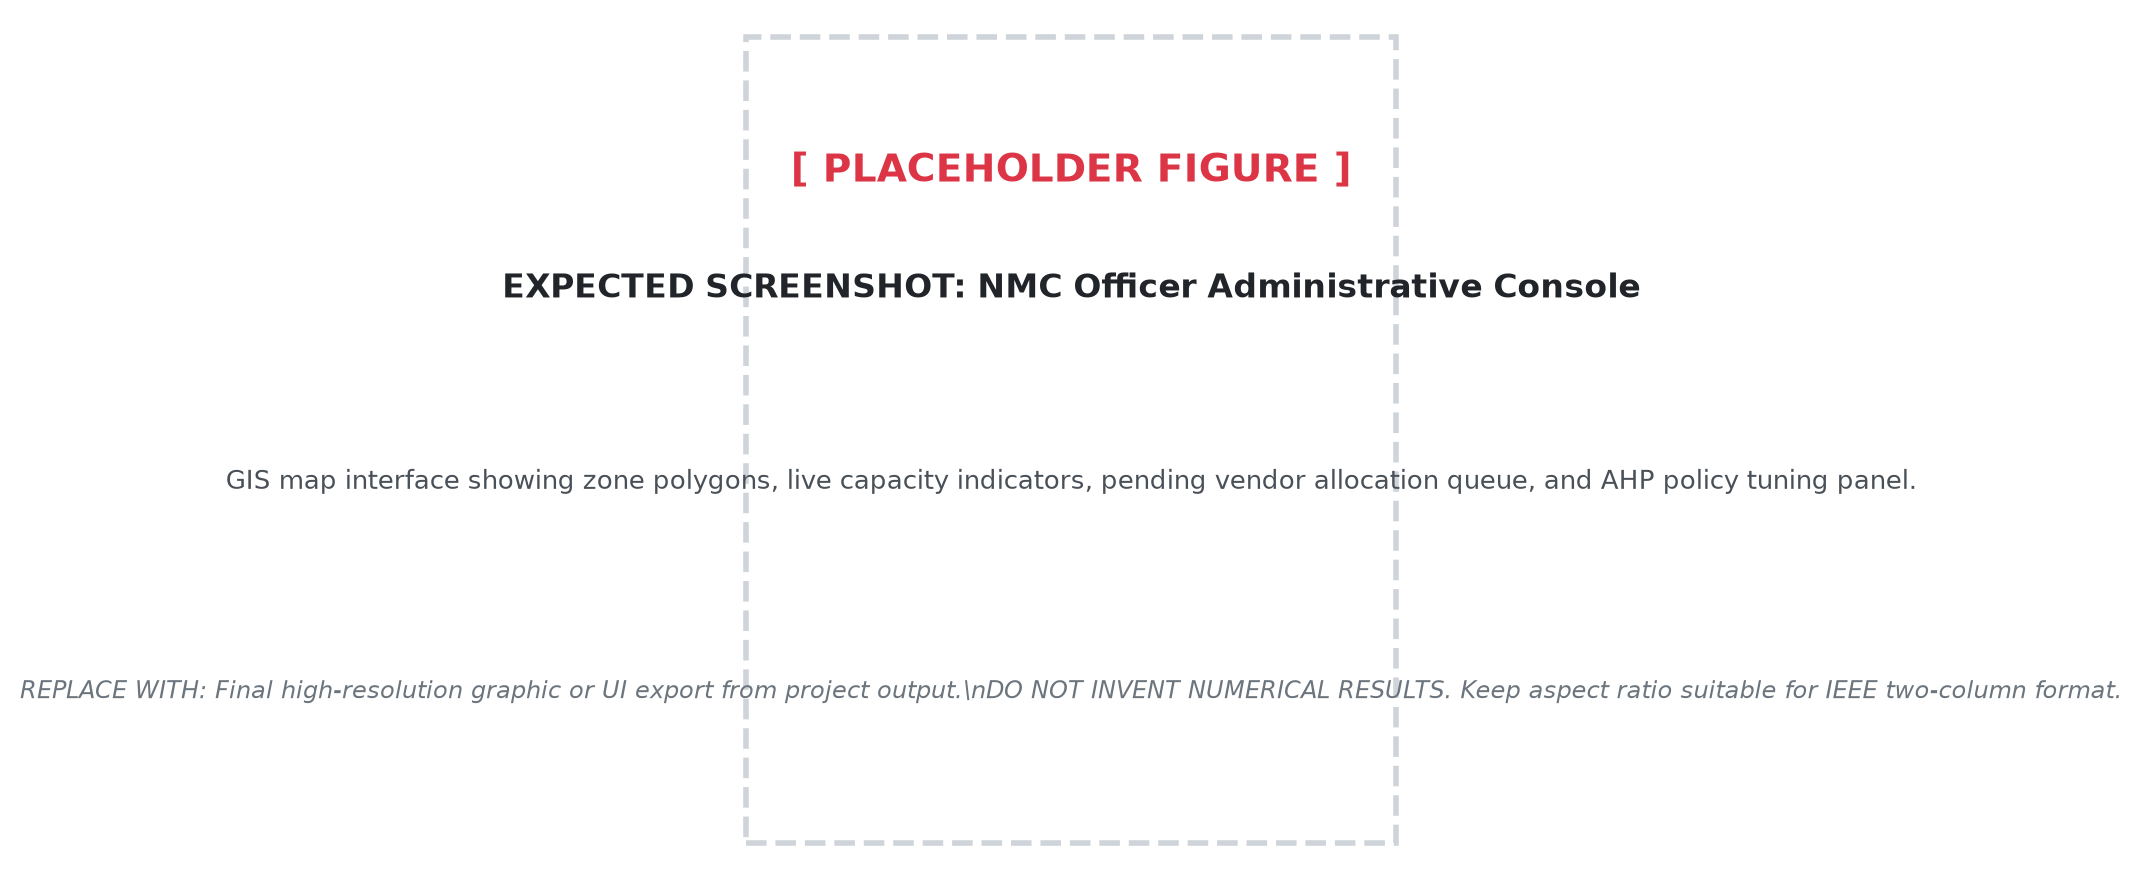
\includegraphics[width=\columnwidth]{figures/placeholders/ui_admin_dashboard_placeholder.png}
    \caption{NMC town-planning officer console showing GIS zone polygons, live capacity indicators, and pending allocation review queues.}
    \label{fig:ui_admin}
\end{figure}

\subsection{Multilingual Vendor Web Portal}
\label{sec:impl_vendor_ui}

To ensure accessibility across linguistic backgrounds, the vendor web portal provides complete internationalization (\texttt{i18n}) supporting both English and Marathi (the regional language of Maharashtra).

\begin{figure}[t]
    \centering
    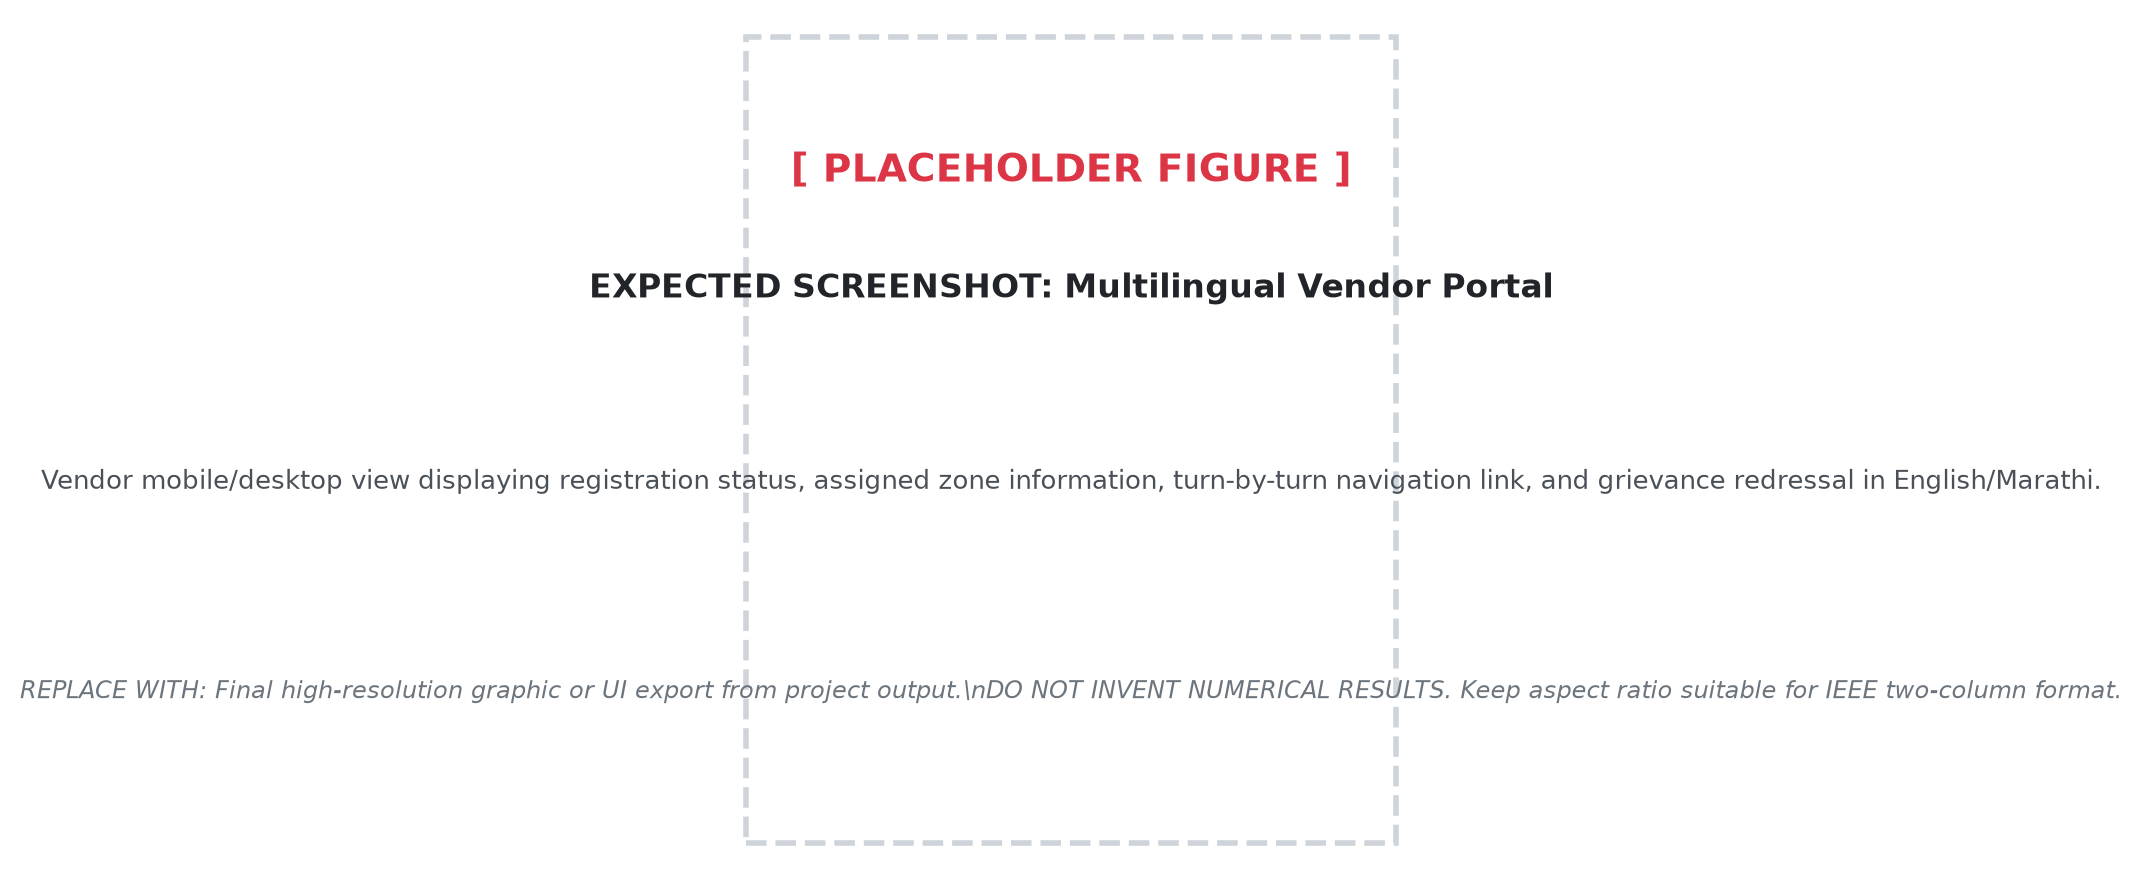
\includegraphics[width=\columnwidth]{figures/placeholders/ui_vendor_portal_placeholder.png}
    \caption{Vendor mobile web portal displaying registration status, assigned zone details, and turn-by-turn navigation guidance in English and Marathi.}
    \label{fig:ui_vendor}
\end{figure}

Key vendor functionalities include:
\begin{itemize}
    \item \textbf{Allocation Status and Digital Credential:} Authenticated vendors can inspect their assigned zone, designated micro-slot identifier (e.g., \texttt{S003}), authorized business category, and permit validity period.
    \item \textbf{Integrated Pedestrian Navigation:} Connects assigned slot coordinates directly to routing engines via Leaflet and GPS geolocators, providing precise turn-by-turn walking directions to the designated $2\,\text{m} \times 2\,\text{m}$ vending footprint.
\end{itemize}

\subsection{Direct Meta WhatsApp Cloud API Conversational Interface}
\label{sec:impl_whatsapp}

Recognizing that many informal vendors face barriers in navigating web browsers or installing mobile applications, UrbanVending AI incorporates an official, direct integration with the Meta WhatsApp Cloud API (Graph API).

\begin{figure}[t]
    \centering
    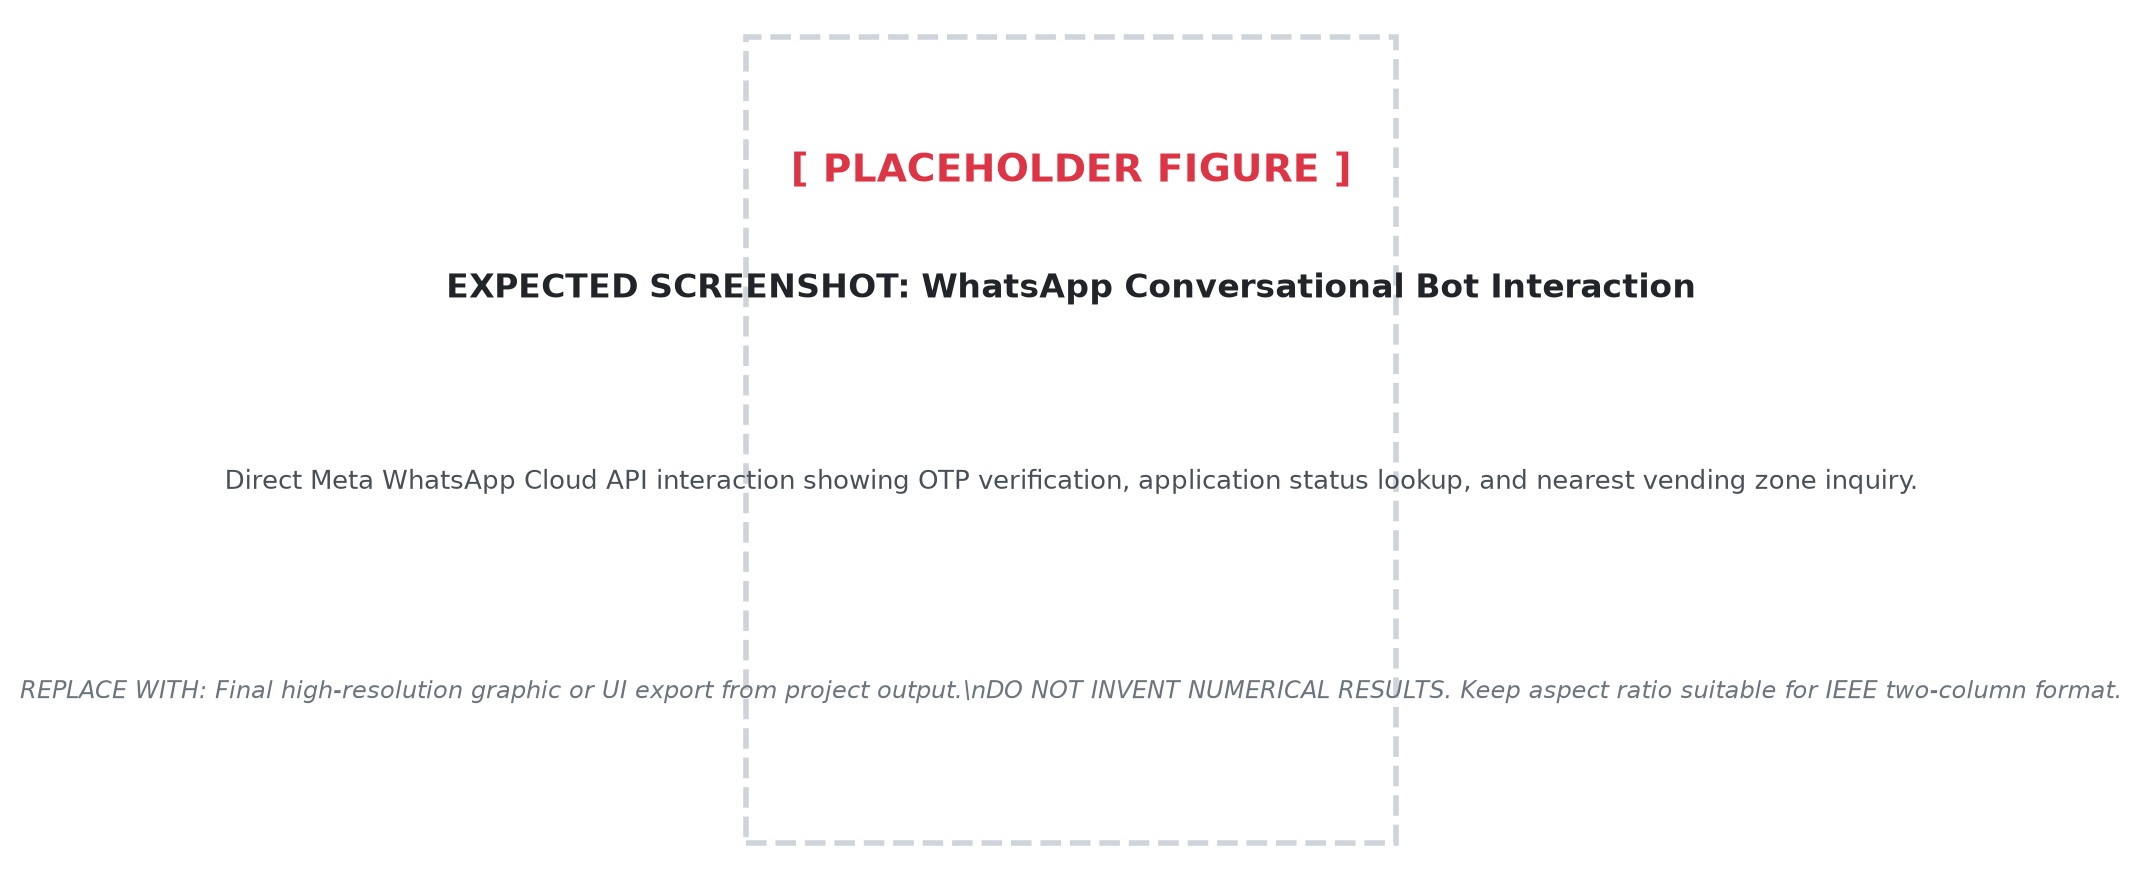
\includegraphics[width=\columnwidth]{figures/placeholders/ui_whatsapp_bot_placeholder.png}
    \caption{Conversational interaction via Meta WhatsApp Cloud API for vendor OTP authentication, status inquiry, and nearby zone discovery.}
    \label{fig:ui_whatsapp}
\end{figure}

The WhatsApp service operates entirely without third-party automation wrappers:
\begin{itemize}
    \item \textbf{Cryptographic Webhook Validation:} Inbound notifications from Meta are verified using HMAC-SHA256 signatures evaluated against \texttt{META\_APP\_SECRET} via the \texttt{X-Hub-Signature-256} header.
    \item \textbf{Persistent Conversational State Machine:} A dedicated conversation state engine in SQLite tracks multi-turn dialogue, enabling vendors to request OTP verification, check application status, locate nearest eligible zones, and register grievances via natural chat interactions.
    \item \textbf{Idempotent Message Deduplication:} Inbound message IDs are deduplicated to prevent double-processing under network retries.
\end{itemize}

\section{Discussion}
\label{sec:discussion}

The development and empirical evaluation of UrbanVending AI provide substantive insights into the intersection of spatial decision analysis, algorithmic fairness, and municipal informal economy governance. This section discusses key findings, practical policy implications, and academic limitations.

\subsection{Key Findings and Methodological Insights}
\label{sec:disc_findings}

The experimental results yield three foundational insights:
\begin{enumerate}
    \item \textbf{Non-linear Scaling Insulates MCDA Against Stakeholder Disagreement:} A common objection to multi-criteria models in municipal governance is that stakeholders cannot agree on objective factor weights. The 224-scenario sensitivity analysis established that when input features undergo non-linear diminishing-returns saturation and exponential proximity decay, the resulting ranking exhibits extreme resilience ($\rho = 0.9977$ mean rank correlation and 100\% Top-1 stability). Consequently, minor policy debates over exact AHP weights do not compromise core zone recommendations.
    \item \textbf{The Inadequacy of Standalone Suitability Ranking:} The case study in Section~\ref{sec:res_paradox} demonstrated that unconstrained suitability ranking produces catastrophic over-allocation in high-density retail corridors (e.g., 50 vendors assigned to a 5-capacity zone). Purely predictive machine learning or greedy ranking models optimize individual vendor placement but ignore collective physical spatial carrying capacity. Two-stage pre-emptive Goal Programming is therefore non-negotiable for real-world municipal feasibility.
    \item \textbf{The Micro-Scale Operational Gap:} High-level town-planning zoning frequently fails during field enforcement because officers and vendors lack micro-spatial certainty. By introducing automated $2\,\text{m} \times 2\,\text{m}$ metric slot generation with sub-millimeter geometric precision ($1.87 \times 10^{-9}\,\text{m}$ error) and guaranteed $1.2\,\text{m}$ pedestrian corridors, UrbanVending AI operationalizes rights-of-way protection without relying on ad-hoc physical demarcation.
\end{enumerate}

\subsection{Policy and Urban Governance Implications}
\label{sec:disc_policy}

UrbanVending AI directly supports the implementation of statutory mandates under the \textit{Street Vendors Act, 2014}~\cite{india2014street}. Specifically:
\begin{itemize}
    \item \textbf{Town Vending Committee (TVC) Empowerment:} The AHP calibration panel provides TVC members—comprising municipal authorities, police representatives, and vendor union leaders—with a transparent mathematical forum to establish consensus weights while monitoring consistency ratios ($CR \le 0.10$).
    \item \textbf{Digital Inclusivity and Anti-Extortion Safeguards:} By delivering digital allocation credentials and navigation guidance directly through the Meta WhatsApp Cloud API in Marathi and English, the platform removes informational gatekeeping, protecting vulnerable informal vendors from harassment and unauthorized middleman fees.
    \item \textbf{Auditable Livelihood Protection:} Every allocation decision is logged with full MCDA factor breakdowns and Goal Programming optimization histories, providing an immutable audit trail to defend municipal policies during judicial review or administrative appeals.
\end{itemize}

\subsection{Limitations and Threats to Validity}
\label{sec:disc_limitations}

In adherence to research integrity, several limitations of the present study must be explicitly acknowledged:
\begin{enumerate}
    \item \textbf{Volunteer Geographic Information (OSM) Incompleteness:} Although OpenStreetMap provided 13,988 road links and 353 commercial POIs, crowdsourced spatial data in Indian tier-two cities exhibits geographic unevenness. An observed zero POI count in a newly developing peripheral ward does not establish the physical absence of informal commerce.
    \item \textbf{Unmapped Municipal Geometries:} While 258 official zones possessed usable spatial boundaries, 50 zones in the official NMC registry lacked geographic coordinates and could not be evaluated. Complete citywide coverage requires physical municipal re-surveys.
    \item \textbf{Supervised Suitability Dataset Constraints:} The supervised machine learning and TreeSHAP models benchmarked in Section~\ref{sec:res_ml_shap} evaluated 140 instances. While grouped cross-validation prevented leakage, the supervised models represent an experimental proof-of-pipeline. Institutional deployment should continue to rely on the transparent AHP-MCDA engine until large-scale, multi-year empirical business revenue outcomes are collected.
    \item \textbf{Static vs. Temporal Vending Dynamics:} The current framework models spatial capacity statically. However, street vending often exhibits intense temporal cyclicity (e.g., morning fresh vegetable markets transitioning to evening street food hubs). Temporal time-banking of micro-slots represents an important area for subsequent development.
\end{enumerate}

\section{Conclusion and Future Scope}
\label{sec:conclusion}

This paper presented \textbf{UrbanVending AI}, an end-to-end geospatial decision-support and micro-allocation framework engineered to resolve the long-standing tension between municipal street vendor livelihood protection and urban right-of-way management. Grounded in statutory mandates under the \textit{Street Vendors Act, 2014}, the proposed seven-stage framework unifies multi-source GIS feature engineering, unsupervised environmental typology clustering, missing-data-aware MCDA, AHP consistency calibration, two-stage pre-emptive Goal Programming, and metric micro-slot packing.

Evaluated on official datasets from the Nashik Municipal Corporation (NMC) encompassing 7,259 registered vendors and 308 municipal zones cross-referenced with 13,988 OpenStreetMap road geometries, the framework demonstrated exceptional technical performance:
\begin{itemize}
    \item \textbf{MCDA Robustness:} Across 224 weight-perturbation scenarios, the multi-criteria engine achieved 100\% Top-1 ranking stability and a mean Spearman rank correlation of $\rho = 0.9977$.
    \item \textbf{Constrained Allocation:} The HiGHS Goal Programming solver eliminated the spatial over-allocation paradox, enforcing hard capacity ceilings while legally placing the maximum feasible vendor population.
    \item \textbf{Physical Micro-Allocation:} Validated on the Lekha Nagar pilot (Zone \texttt{NN\_F\_013}), the metric slot generator packed 10 standardized $2\,\text{m} \times 2\,\text{m}$ vending footprints ($1.87 \times 10^{-9}\,\text{m}$ maximum edge error) while preserving an uninterrupted $1.20\,\text{m}$ pedestrian clearance corridor.
    \item \textbf{Attribution Transparency:} Supervised benchmarking demonstrated that Random Forest regression ($R^2 = 0.7592$, $\text{MAE} = 0.2469$) achieved a 59.8\% error reduction over baselines, with TreeSHAP attributions verifying that commercial footfall and education facilities represent primary suitability drivers.
    \item \textbf{Operational Privacy:} The full-stack deployment incorporates cryptographic HMAC-SHA256 identity hashing and direct Meta WhatsApp Cloud API integration, delivering transparent municipal services directly to informal workers without privacy compromise.
\end{itemize}

\subsection{Future Work}
\label{sec:future_work}

Future enhancements will target four promising directions:
\begin{enumerate}
    \item \textbf{Temporal Micro-Slot Time-Banking:} Extending the Goal Programming model to incorporate dynamic temporal constraints, enabling multiple vendors (e.g., morning agricultural producers and evening food caterers) to share the same physical $2\,\text{m}\times 2\,\text{m}$ footprint across distinct diurnal shifts.
    \item \textbf{High-Resolution Aerial and Mobile LiDAR Surveys:} Deploying drone-based photogrammetry and vehicle-mounted LiDAR to map the 50 currently unmapped municipal zones and automate sidewalk obstruction detection.
    \item \textbf{Longitudinal Socioeconomic Impact Evaluation:} Conducting multi-year field surveys across pilot zones to quantify the direct impact of algorithmic allocation on vendor daily earnings, customer footfall, and municipal permit revenue.
    \item \textbf{Generalization Across Diverse Municipalities:} Validating the transferability of the UrbanVending AI framework across diverse urban contexts and metropolitan municipal corporations across India.
\end{enumerate}


% ---------------------------------------------------------------------------
% Bibliography
% ---------------------------------------------------------------------------
\bibliographystyle{IEEEtran}
\bibliography{references}

\end{document}
